\exercisesection{1}

\begin{enumerate}
\def\labelenumi{\arabic{enumi}.}
\tightlist
\item
  \begin{enumerate}
  \def\labelenumii{(\alph{enumii})}
  \tightlist
  \item
    设 A 是绝对平坦环（第 I 章，§2，习题 17）。证明 Ass(A) 是 Spec(A) 的孤立点组成的集（注意 Ass(A) 是 A 的幂等元的零化子这样的素理想组成的集）。
  \end{enumerate}
\end{enumerate}

\begin{enumerate}
\def\labelenumi{(\alph{enumi})}
\setcounter{enumi}{1}
\item
  由 (a) 推出一个环 A 的例子，使 \(A \neq 0\) 且 \(\operatorname{Ass}(A) = \varnothing\) （参见第 II 章，§4，习题 17），并且第 1 节命题 2 的推论 2 的结论对它不成立。
\item
  由 (b) 推出一个环 A 及 A 的乘性子集 S 的例子，使得 \(p \mapsto S^{-1}p\) 这一从 \(\text{Ass}(A) \cap \Phi\) 到 \(\text{Ass}(S^{-1}A)\) 的映射（第 2 节，命题 5）不是满射。
\end{enumerate}

* 2. 设 K 是交换域，A 是以 Q 为阶群的赋值环，由``形式幂级数'' \(\sum_{r} c_r T^r\) 组成，其中 \(c_r \in K\) ，\(r \in \mathbf{Q}_+\) ，且诸 \(r\) 中使 \(c_r \neq 0\) 者所成的集是良序的。设 \(\alpha\) 是无理数 \(>0\) ，\(a\) 是 A 中由赋值 \(>\alpha\) 的元素组成的理想，C 是环 A/a。那么 \(\text{Spec(C)}\) 只剩一点 \(p\) ；对 C 中所有 \(x \neq 0\) ，有 \(px \neq 0\) ，但对所有 \(\lambda \in p\) ，存在 C 中的 \(y \neq 0\) 使 \(\lambda y = 0\) 。特别地，\(\text{Ass(C)} = \varnothing\) ，尽管 \(\text{Supp(C)} = \text{Spec(C)} = \{\mathfrak{p}\}\) 。 *

\begin{enumerate}
\def\labelenumi{\arabic{enumi}.}
\setcounter{enumi}{2}
\item
  设 M 是 A-模，N 是 M 的子模。证明每个不包含 Ann(N) 的素理想 \(\mathfrak{p} \in \operatorname{Ass}(M/N)\) 都伴随于 M。给出一个属于 Ass(M/N) 而不属于 Ass(M) 的理想 p 的例子（取 A 为整环，M = A）。
\item
  给出一个环 A 的例子，使 M = A 不满足第 4 节定理 1 的结论（参见习题 1 (b)）。
\item
  设 A = K{[}X, Y{]} 是交换域 K 上两个未定元的多项式代数，a 是 A 的极大理想 AX + AY。证明 \(\text{Supp}(a) = \text{Spec}(A)\) 是无限集，且 \(\text{Ass}(a) = \{0\}\) 。证明 a 没有所有因子模都与 A 同构的合成列。（这样的列的存在将意味着 a 同构于某个模 \(A^{n}\) ；于是必有 n = 1，这是荒谬的。）
\end{enumerate}

¶ 6. 设 A 是环，E 是 A-模。

\begin{enumerate}
\def\labelenumi{(\alph{enumi})}
\item
  证明：要使 A 的素理想 p 属于 Supp(E)，必须且只需存在 E 的子模 F 使 \(p \in \text{Ass}(E/F)\) （要证条件必要，考虑 E 中形如 px 的子模 F，其中 \(x \in E\) ；要证条件充分，用第 3 节命题 7）。
\item
  假设 A 是 Noether 环且 E 有限生成。证明对每个素理想 \(\mathfrak{p}\in\operatorname{Supp}(\mathrm{E})\) ，存在 E 的合成列 \((\mathrm{E}_{i})_{0\leqslant i\leqslant n}\) ，使得对 \(0\leqslant i\leqslant n-1\) ，\(E_{i}/E_{i+1}\) 同构于 \(A/p_{i}\) ，其中 \(p_{i}\) 是素理想，且诸 \(p_{i}\) 中有一个等于 p。
\end{enumerate}

\begin{enumerate}
\def\labelenumi{\arabic{enumi}.}
\setcounter{enumi}{6}
\tightlist
\item
  设 A 是 Noether 环，M 是有限生成 A-模，\(\mathfrak{a} = \text{Ann}(M)\) 。
\end{enumerate}

\begin{enumerate}
\def\labelenumi{(\alph{enumi})}
\item
  证明：若 \(\mathfrak{a}\) 是素的，则 \(\mathfrak{a}\) 是 \(\operatorname{Ass}(\mathbf{M})\) 的最小元。（注意 \(\mathfrak{a} = \bigcap_{\mathfrak{p} \in \operatorname{Ass}(\mathbf{M})} \mathfrak{p}\) 。）
\item
  证明伴随于 A/a 的每个素理想都伴随于 M。（注意若 p 是 A 的素理想，且是元素 \(\alpha \in A\) 在 A/a 中的类的零化子，则 \(\mathfrak{p} = \operatorname{Ann}(\alpha\mathbf{M})\) ，然后用 (a)。）
\item
  设 \(p, q\) 是 \(A\) 的两个不同的素理想，满足 \(p \subset q\) 。证明：若 \(M = (A/p) \oplus (A/q)\) ，则 \(\operatorname{Ass}(A/a) \neq \operatorname{Ass}(M)\) 。
\end{enumerate}

\begin{enumerate}
\def\labelenumi{\arabic{enumi}.}
\setcounter{enumi}{7}
\item
  设 A 是 Noether 环，a 是 A 的理想，M 是有限生成 A-模，P 是 M 中由满足 ax = 0 的 \(x \in M\) 组成的子模。证明 \(\operatorname{Ass}(M/P) \subset \operatorname{Ass}(M)\) （注意对每个 \(x \in M\) ，\((Ax + P)/P\) 的零化子也是 ax 的零化子，并用习题 7 (a)）。
\item
  设 A 是 Noether 环，a 是 A 的理想。
\end{enumerate}

\begin{enumerate}
\def\labelenumi{(\alph{enumi})}
\item
  要使 A 的理想 b 满足 a: b ≠ a，必须且只需 b 含于某个素理想 p ∈ Ass(A/a)。
\item
  设 A 是域 K 上 3 个未定元的多项式代数 K{[}X, Y, Z{]}。设 n = AX，m = AX + AY + AZ，a = n ∩ m²。证明存在包含 a 的素理想 p 使 a: p ≠ a，但它不伴随于 A。
\end{enumerate}

\begin{enumerate}
\def\labelenumi{\arabic{enumi}.}
\setcounter{enumi}{9}
\tightlist
\item
  \begin{enumerate}
  \def\labelenumii{(\alph{enumii})}
  \tightlist
  \item
    给出一个 Z-模 M 的例子，使 \(\operatorname{Ass}(\operatorname{Hom}_{\mathbf{Z}}(\mathbf{M}, \mathbf{M}))\) 不含于 \(\operatorname{Supp}(\mathbf{M})\) （参见第 II 章，§ 4，习题 24 (c)）。
  \end{enumerate}
\end{enumerate}

\begin{enumerate}
\def\labelenumi{(\alph{enumi})}
\setcounter{enumi}{1}
\tightlist
\item
  给出 Z-模 E、F 的例子，使得
\end{enumerate}

\[
\operatorname{Ass} \left(\operatorname{Hom} _ {\mathbf {Z}} (\mathrm{E}, \mathrm{F})\right) = \varnothing ,
\]

但 \(\operatorname{Ass}(\mathbf{F}) \cap \operatorname{Supp}(\mathbf{E}) \neq \varnothing\) （取 \(\mathbf{F} = \mathbf{Z}\) ）。

\begin{enumerate}
\def\labelenumi{\arabic{enumi}.}
\setcounter{enumi}{10}
\tightlist
\item
  \begin{enumerate}
  \def\labelenumii{(\alph{enumii})}
  \tightlist
  \item
    设 \(\mathbf{A}\) 是 Noether 环，\(\mathbf{E}\) 是 \(\mathbf{A}\) -模。证明从 E 到乘积 \(\prod_{p\in\text{Ass}(E)}E_p\) 的典范同态是单射（若 N 是这个同态的核，证明 \(\text{Ass}(N)=\varnothing\) ）。
  \end{enumerate}
\end{enumerate}

\begin{enumerate}
\def\labelenumi{(\alph{enumi})}
\setcounter{enumi}{1}
\tightlist
\item
  取 A 为域 K 上的多项式环 K{[}X,Y,Z{]}；设 \(p_{1}=AX+AY\) ，\(p_{2}=AX+AZ\) ，它们是素理想，又设 a 为理想 \(p_{1}p_{2}\) 。集合 \(\operatorname{Ass}(A/a)\) 由 \(p_{1}\) 、\(p_{2}\) 及极大理想 \(m=p_{1}+p_{2}\) 组成；证明从 E=A/a 到 \(E_{p_{1}}\times E_{p_{2}}\) 的典范同态不是单射。
\end{enumerate}

\begin{enumerate}
\def\labelenumi{\arabic{enumi}.}
\setcounter{enumi}{11}
\tightlist
\item
  设 A 是 Noether 环，P 是投射 A-模。证明：若对每个 \(p \in \text{Ass}(A)\) ，\(P_{p}\) 都是有限生成 \(A_{p}\) -模，则 P 是有限生成 A-模（把 A 嵌入乘积 \(\prod_{p \in \text{Ass}(A)} A_{p}\) （习题 11），并用《代数》第 II 章，§ 5，第 5 节，命题 9）。
\end{enumerate}

¶ 13. 设 A 是 Noether 环，E 是有限生成 A-模，p、q 是 A 的两个素理想，满足 \(p \subset q\) ，a 是 q 的一个元素。假设 \(p \in \text{Ass}(E)\) 且位似映射 \(a_{E}\) 是单射。证明存在素理想 \(n \in \text{Ass}(E/aE)\) 使 \(p + Aa \subset n \subset q\) 。（把 A 换成 \(A_{q}\) ，可设 A 是以 q 为极大理想的局部环。设 \(F \neq 0\) 是 E 中由满足 px = 0 的 x 组成的子模。证明关系 \(F \subset aE\) 将导出 F = aF，并用 Nakayama 引理得出矛盾。然后用第 4 节命题 8。）

\begin{enumerate}
\def\labelenumi{\arabic{enumi}.}
\setcounter{enumi}{13}
\item
  设 A 是整环，\(a \neq 0\) 是 A 的元素，p 是 \(\operatorname{Ass}(A/aA)\) 的元素。证明对 p 的每个元素 \(b \neq 0\) ，有 \(\mathfrak{p} \in \operatorname{Ass}(A/bA)\) （若 \(c \in A\) 使关系 \(xc \in aA\) 等价于 \(x \in p\) ，证明存在 \(d \in A\) 使 \(xd \in bA\) 等价于 \(xc \in aA\) ）。
\item
  设 A 是 Noether 环，E 是有限生成 A-模，F 是 E 的子模，m 是 A 的理想。要使 F 在 E 中对于 m-进拓扑是闭的，必须且只需 \(p + m \neq A\) 对每个理想 \(p \in \text{Ass}(E/F)\) 成立。（化归到 F = 0 的情形，用第 III 章，§3，第 2 节，命题 5 的推论，并把第 1 节命题 2 的推论 2 应用于元素 \(1 + m\) ，其中 \(m \in m\) 。）
\item
  设 A 是 Noether 环。要使 A 同构于有限多个整环的乘积，必须且只需对 A 的每个素理想 p，局部环 \(A_{p}\) 都是整环。（要证条件充分，首先注意它蕴涵环 A 是约化的；由此推出 \(\{0\} = \bigcap_{i} p_{i}\) ，其中 \(p_{i} (1 \leqslant i \leqslant n)\) 是 A 的极小素理想。证明对 \(i \neq j\) ，必有 \(p_{i} + p_{j} = A\) ；为此注意，若存在包含 \(p_{i} + p_{j}\) 的极大理想 m，则环 \(A_{m}\) 就不是整环，这里要用第 1 节命题 2 的推论 3 及第 2 节命题 5 的推论。）
\end{enumerate}

¶ 17. 设 A 是环，M 是 A-模。若存在 \(x \in \mathbf{M}\) 使 p 是包含 Ann(x) 的素理想组成的集的极小元，则称 A 的素理想 p 弱伴随于 M；我们用 \(\operatorname{Ass}_{f}(\mathbf{M})\) 表示弱伴随于 M 的理想组成的集。那么 \(\operatorname{Ass}(\mathbf{M}) \subset \operatorname{Ass}_{f}(\mathbf{M})\) 。

\begin{enumerate}
\def\labelenumi{(\alph{enumi})}
\item
  证明关系 \(\mathbf{M} \neq 0\) 等价于 \(\operatorname{Ass}_f(\mathbf{M}) \neq \varnothing\) 。
\item
  要使 \(a \in \mathbf{A}\) 满足 \(a_{\mathbf{M}}\) 是单射，必须且只需 \(a\) 不属于 \(\operatorname{Ass}_f(\mathbf{M})\) 的任何元素（注意，若 \(a\) 属于某个理想 \(\operatorname{Ann}(x)\) 的根，其中 \(x \neq 0\) 在 \(\mathbf{M}\) 中，则存在 \(y \neq 0\) 于 \(\mathbf{M}\) 中，使 \(a \in \operatorname{Ann}(y)\) 。要证条件必要，考虑环 \(\operatorname{A}/\operatorname{Ann}(x)\) ，把它化为证明：在环 \(\mathbf{A}\) 中，属于素理想 \(p\) （它在 \(\mathbf{A}\) 的素理想组成的集中极小）的每个元素必是零因子（第 II 章，§ 2，第 6 节，命题 12）。）
\end{enumerate}

要使 \(a \in A\) 满足 \(a_{M}\) 是殆幂零的，必须且只需 a 属于 \(\operatorname{Ass}_{f}(M)\) 的所有元素。

\begin{enumerate}
\def\labelenumi{(\alph{enumi})}
\setcounter{enumi}{2}
\tightlist
\item
  若 \(\mathbf{N}\) 是 \(\mathbf{M}\) 的子模，则
\end{enumerate}

\[
\operatorname{Ass} _ {f} (\mathbf {N}) \subset \operatorname{Ass} _ {f} (\mathbf {M}) \subset \operatorname{Ass} _ {f} (\mathbf {N}) \cup \operatorname{Ass} _ {f} (\mathbf {M} / \mathbf {N}).
\]

（注意，若 \(\mathfrak{p}\) 是素理想，\(a \notin \mathfrak{p}\) ，\(x \in \mathbf{M}\) 满足 \(ax \in \mathbf{N}\) 且 \(\operatorname{Ann}(x) \subset \mathfrak{p}\) ，则 \(\operatorname{Ann}(ax) \subset \mathfrak{p}\) 。）

\begin{enumerate}
\def\labelenumi{(\alph{enumi})}
\setcounter{enumi}{3}
\item
  设 S 是 A 的乘性子集，\(\Phi\) 是 A 中与 S 不相交的素理想组成的集。证明 \(p \mapsto S^{-1}p\) 是从 \(\operatorname{Ass}_{f}(M) \cap \Phi\) 到 \(\operatorname{Ass}_{f}(S^{-1}M)\) 上的双射。（注意，在典范映射 \(A \to S^{-1}A\) 下，元素 x/s（其中 \(x \in M\) ，\(s \in S\) ）的零化子的原像是 \(\operatorname{Ann}(x)\) 关于 S 的饱和。）
\item
  设 S 是 A 的乘性子集；证明：若 N 是典范同态 \(M \to S^{-1}M\) 的核，则 \(\operatorname{Ass}_{f}(N)\) 是由 \(p \in \operatorname{Ass}_{f}(M)\) 中与 S 相交者组成的集，而 \(\operatorname{Ass}_{f}(M/N)\) 是由 \(p \in \operatorname{Ass}_{f}(M)\) 中与 S 不相交者组成的集。（为证后一点，考虑在包含 \(\operatorname{Ann}(\bar{y})\) 的理想中极小的素理想 q，其中 \(\bar{y} \in M/N\) ；注意，若 \(y \in \bar{y}\) 且 \(t \in q\) ，则存在 \(c \notin q\) 及整数 n \textgreater{} 0 使 \(ct^{n}y \in N\) （第 II 章，§2，第 6 节，命题 12）；先由此推出 \(q \cap S = \varnothing\) 。存在 \(s \in S\) 使 \(sct^{n}y = 0\) ；由此断定不可能有素理想 \(q' \neq q\) 使 \(\operatorname{Ann}(y) \subset q' \subset q\) 。）
\item
  要使 \(\mathbf{A}\) 的素理想属于 \(\operatorname{Supp}(\mathbf{M})\) ，必须且只需它包含 \(\operatorname{Ass}_f(\mathbf{M})\) 的一个元素。
\item
  证明：若 A 是 Noether 环，则 \(\operatorname{Ass}_f(M) = \operatorname{Ass}(M)\) 。
\item
  若 \(\mathbf{A}\) 是绝对平坦环，则 \(\operatorname{Ass}_f(\mathbf{A}) = \operatorname{Spec}(\mathbf{A})\) 。
\item
  对每个 A-模 E，从 E 到乘积
\end{enumerate}

\(\prod_{p\in\mathrm{Ass}_{f}(\mathbf{E})}\mathrm{E}_{p}\) 的典范同态是单射；换言之，\(\{0\}\) 在 E 中关于诸理想 \(p\in\mathrm{Ass}_{f}(\mathbf{E})\) 的饱和的交化为 0。类似地推广习题 12。

\begin{enumerate}
\def\labelenumi{(\alph{enumi})}
\setcounter{enumi}{9}
\tightlist
\item
  设 M 是有限生成 A-模。证明包含 \(\mathfrak{a} = \text{Ann}(M)\) 的素理想组成的集的极小元都属于 \(\text{Ass}_{f}(M)\) （若 \((x_{i})_{1 \leq i \leq n}\) 是 M 的生成系，证明这样的理想包含某个 \(\text{Ann}(x_{i})\) ）。由此推出 \(\text{Ass}_{f}(A/a)\) 含于 \(\text{Ass}_{f}(M)\) （若素理想 p 包含元素 \(\alpha \in A\) 模 a 的类的零化子，注意 p 包含 M 的子模 \(\alpha M\) 的零化子）；证明 \(\text{Ass}_{f}(A/a)\) 、\(\text{Ass}(M)\) 与包含 a 的素理想组成的集有相同的极小元。
\end{enumerate}

\begin{enumerate}
\def\labelenumi{\arabic{enumi}.}
\setcounter{enumi}{17}
\tightlist
\item
  设 A 是环，M 是 A-模。要使元素 \(c \in A\) 满足：对每个 \(a \in A\) （其位似映射 \(a_{M}\) 为单射），\(b_{M}\) 对所有形如 \(a + \lambda c\) （其中 \(\lambda \in A\) ）的 b 都是单射位似映射，只需 c 属于 \(\operatorname{Ass}_{f}(M)\) 的极大元之交（用习题 17 (b)）。这个条件必要吗？
\end{enumerate}

* 19. 设 A 是高为 2 的赋值的环，\(\Gamma\) 是它的阶群，\(\Gamma_1\) 是 \(\Gamma\) 的异于 \(\{0\}\) 与 \(\Gamma\) 的唯一孤立子群，\(\gamma > 0\) 是 \(\Gamma\) 中不属于 \(\Gamma_1\) 的元素。设 \(a\) 是由 \(x \in A\) 中使 \(v(x) \geqslant \gamma\) 的元素组成的理想，\(b\) 是由 \(x \in A\) 中使 \(v(x) > \gamma\) 的元素组成的理想，\(E = A/a\) ，\(F = A/b\) 。证明 \(\operatorname{Ass}_f(\operatorname{Hom}_A(E, F))\) 异于 \(\operatorname{Ass}_f(F) \cap \operatorname{Supp}(E)\) 。 *

\exercisesection{2}

\begin{enumerate}
\def\labelenumi{\arabic{enumi}.}
\tightlist
\item
  \begin{enumerate}
  \def\labelenumii{(\alph{enumii})}
  \tightlist
  \item
    证明在 Noether 多项式环 \(\mathbf{A} = \mathbf{Z}[\mathbf{X}]\) （\(\mathbf{Z}\) 上一个未定元）中，理想 \(m = 2A + AX\) 是极大的，而理想 \(q = 4A + AX\) 是 m-准素的，但不等于 \(m\) 的任何幂。
  \end{enumerate}
\end{enumerate}

\begin{enumerate}
\def\labelenumi{(\alph{enumi})}
\setcounter{enumi}{1}
\item
  在 Noether 环 \(\mathbf{B} = \mathbf{Z}[2\mathbf{X},\mathbf{X}^2,\mathbf{X}^3] \subset \mathbf{A}\) 中，证明理想 \(\mathfrak{p} = 2\mathrm{BX} + \mathrm{BX}^2\) 是素的，但 \(\mathfrak{p}^2\) 不是 \(\mathfrak{p}\) -准素的，尽管它的根等于 \(\mathfrak{p}\) 。
\item
  设 \(\mathbf{K}\) 是交换域，\(\mathbf{A}\) 是 \(\mathbf{K}[\mathbf{X},\mathbf{Y},\mathbf{Z}]\) 模由 \(Z^2 -\mathbf{XY}\) 生成的理想所得的商环；设 \(x,y,z\) 是 \(\mathbf{X},\mathbf{Y},\mathbf{Z}\) 在 \(\mathbf{A}\) 中的典范像。证明 \(\mathfrak{p} = \mathbf{A}x + \mathbf{A}z\) 是素的，\(\mathfrak{p}^2\) 不是准素的，且 \(\mathfrak{p}^2 = \mathfrak{a}\cap \mathfrak{b}^2\) 是 \(\mathfrak{p}^2\) 的一个准素分解，其中 \(\mathfrak{a} = \mathbf{A}x\) ，\(\mathfrak{b} = \mathbf{A}x + \mathbf{A}y + \mathbf{A}z\) 。
\end{enumerate}

\begin{enumerate}
\def\labelenumi{\arabic{enumi}.}
\setcounter{enumi}{1}
\item
  在 §1 习题 11 (b) 的例子中，证明 \(\mathfrak{a} = \mathfrak{m}^2 \cap \mathfrak{p}_1 \cap \mathfrak{p}_2\) 是 \(\mathfrak{a}\) 在 \(\mathbf{A}\) 中的一个既约准素分解，且 \(\mathfrak{a}\) 关于 \(\mathfrak{m}\) 的饱和等于 \(\mathfrak{a}\) （因而不是准素的）。
\item
  设 A 是 Noether 环，M 是有限生成 A-模。设 Q 是 M 中的 p-准素子模。诸整数 \(n \geqslant 1\) 中使 \(p^{n}M \subset Q\) 者的下确界称为 Q 在 M 中的指数，记作 \(e(M/Q)\) 。
\end{enumerate}

设 \((Q_{\lambda})_{\lambda \in L}\) 是 M 中的一族 \(p\) -准素子模。要使 \(Q = \bigcap_{\lambda \in L} Q_{\lambda}\) 在 M 中是 p-准素的，必须且只需族 \((e(\mathbf{M}/\mathbf{Q}_{\lambda}))_{\lambda\in\mathbf{L}}\) 有上界；此时 \(e(\mathbf{M}/\mathbf{Q})\geqslant e(\mathbf{M}/\mathbf{Q}_{\lambda})\) 对所有 \(\lambda\in L\) 成立。

¶ 4. 设 A 是 Noether 环，M 是有限生成 A-模。设 p 是 Ass(M) 的元素，\(\mathfrak{G}_{\mathfrak{p}}\) 是 M 中满足 \(\operatorname{Ass}(M/Q) = \{\mathfrak{p}\}\) 且 \(\operatorname{Ass}(Q) = \operatorname{Ass}(M) - \{\mathfrak{p}\}\) 的子模 Q 组成的集（由 § 1 第 1 节命题 4，这个集非空）。我们写 \(e_{\mathfrak{p}}(M) = \inf_{\mathbf{Q} \in \mathfrak{G}_{\mathfrak{p}}} e(M/Q)\) （习题 3）。

\begin{enumerate}
\def\labelenumi{(\alph{enumi})}
\item
  设 \(n_{\mathfrak{p}}\) 是整数 \(\geqslant e_{\mathfrak{p}}(\mathbf{M})\) ，\(\mathfrak{F}(n_{\mathfrak{p}})\) 是 \(\mathfrak{G}_{\mathfrak{p}}\) 中由子模 \(\mathbf{Q}\) 之使 \(e(\mathbf{M} / \mathbf{Q}) \leqslant n_{\mathfrak{p}}\) 者组成的子集。证明 \(\mathfrak{F}(n_{\mathfrak{p}})\) 有最小元 \(\mathbf{Q}(\mathfrak{p}, n_{\mathfrak{p}})\) 。
\item
  设 \((n_{\mathfrak{p}})_{\mathfrak{p} \in \operatorname{Ass}(\mathbf{M})}\) 是一族整数，使 \(n_{\mathfrak{p}} \geqslant e_{\mathfrak{p}}(\mathbf{M})\) 对所有 \(\mathfrak{p} \in \operatorname{Ass}(\mathbf{M})\) 成立。证明与这个族相应的诸子模 \(\mathbf{Q}(\mathfrak{p}, n_{\mathfrak{p}})\) 构成 \(\{0\}\) 在 \(\mathbf{M}\) 中的一个由族 \((n_{\mathfrak{p}})\) 典范确定的既约准素分解。若取 \(n_{\mathfrak{p}} = e_{\mathfrak{p}}(\mathbf{M})\) （对所有 \(\mathfrak{p} \in \operatorname{Ass}(\mathbf{M})\) ），则由诸 \(\mathbf{Q}(\mathfrak{p}) = \mathbf{Q}(\mathfrak{p}, e_{\mathfrak{p}}(\mathbf{M}))\) 组成的准素分解称为 \(\{0\}\) 在 \(\mathbf{M}\) 中的典范准素分解。设 \(\{0\} = \bigcap_{\mathfrak{p} \in \operatorname{Ass}(\mathbf{M})} \mathbf{Q}'(\mathfrak{p})\) 是 \(\{0\}\) 在 \(\mathbf{M}\) 中的任意一个既约准素分解。证明 \(e(\mathbf{M}/\mathbf{Q}(\mathfrak{p})) \leqslant e(\mathbf{M}/\mathbf{Q}'(\mathfrak{p}))\) 对所有 \(\mathfrak{p} \in \operatorname{Ass}(\mathbf{M})\) 成立，且若 \(e(\mathbf{M}/\mathbf{Q}(\mathfrak{p})) = e(\mathbf{M}/\mathbf{Q}'(\mathfrak{p}))\) 对某个 \(\mathfrak{p}\) 成立，则 \(\mathbf{Q}(\mathfrak{p}) \subset \mathbf{Q}'(\mathfrak{p})\) （``Ortiz 定理''）。
\item
  证明 \(\mathbf{Q}(\mathfrak{p}, n_{\mathfrak{p}})\) 是 \(\mathfrak{p}^{n_{\mathfrak{p}}} \mathbf{M}\) 关于 \(\mathfrak{p}\) 的饱和（用 § 1 第 2 节命题 6）；\(\mathfrak{p}\) 是 \(\operatorname{Supp}(\mathbf{M} / \mathfrak{p}^n\mathbf{M})\) 的最小元。
\item
  设 S 是 A 的乘性子集，不与素理想 \(\mathfrak{p} \in \operatorname{Ass}(M)\) 相交，Q 是 M 的 p-准素子模。证明 \(e(\mathrm{M}/\mathrm{Q}) = e(\mathrm{S}^{-1}\mathrm{M}/\mathrm{S}^{-1}\mathrm{Q})\) 。证明：若 S 是 A 的乘性子集，\(\Phi\) 是由 \(\mathfrak{p} \in \operatorname{Ass}(M)\) 中使 \(S \cap \mathfrak{p} = \varnothing\) 者组成的集，N 是 \(\{0\}\) 在 M 中关于 S 的饱和，则诸 \(\mathrm{Q}(\mathfrak{p}, n_{\mathfrak{p}})\) （其中 \(\mathfrak{p} \in \Phi\) ）构成 N 在 M 中由族 \((n_{\mathfrak{p}})_{\mathfrak{p} \in \Phi}\) 典范确定的既约准素分解，而诸 \(S^{-1}\mathrm{Q}(\mathfrak{p}, n_{\mathfrak{p}})\) （其中 \(\mathfrak{p} \in \Phi\) ）构成 \(\{0\}\) 在 \(S^{-1}M\) 中由族 \((n_{\mathfrak{p}})_{\mathfrak{p} \in \Phi}\) 典范确定的既约准素分解。考察典范准素分解这一特殊情形。
\end{enumerate}

\begin{enumerate}
\def\labelenumi{\arabic{enumi}.}
\setcounter{enumi}{4}
\item
  设 L 是有限生成的自由 Z-模，T 是阶为素数 p 的幂的有限交换群。证明 \(\{0\}\) 在 \(M = L \oplus T\) 中的典范准素分解（习题 4）是 \(\{0\} = p^{n}L \cap T\) ，其中 n 是最小整数 \(\geqslant 0\) ，使得 \(p^{n}T = 0\) （注意 \(p^{n}M = p^{n}L\) ）。
\item
  在 § 1 习题 5 中，\{0\} 在 A-模 a 中关于 A 的素理想 \{0\} 是准素的。证明 a 的子模 AX 在 a 中关于某个素理想 \(\neq\{0\}\) 是准素的，而 a 的子模 AXY 在 a 中不是准素的。
\item
  设 \(\mathbf{A}\) 是 Noether 环，\(\mathbf{M}\) 是有限生成 A-模，\((\mathfrak{p}_i)_{1\leqslant i\leqslant n}\) 是把 \(\operatorname {Ass}(\mathbf{M})\) 的元素按任意次序排列所得的序列。证明存在一条合成列 \((\mathbf{M}_i)_{0\leqslant i\leqslant n}\) （\(\mathbf{M}\) 的），使得对 \(0\leqslant i\leqslant n - 1\) ，\(\mathbf{M}_{i + 1}\) 是一个 \(p_i\) -准素子模，位于 \(\mathbf{M}_i\) 中（用第 3 节命题 4）。
\end{enumerate}

¶ 8. 设 A 是 Noether 环，E 是有限生成 A-模，F 是 E 的子模，m 是 A 的理想。设 \(\mathbf{F} = \bigcap_{\mathfrak{p} \in \operatorname{Ass}(\mathbf{E}/\mathbf{F})} \mathbf{Q}(\mathfrak{p})\) 是 F 在 E 中的一个既约准素分解。证明 F 在 E 中对于 E 上的 m-进拓扑的闭包等于 \(\bigcap_{\mathfrak{p} \in \Phi} \mathbf{Q}(\mathfrak{p})\) ，其中 \(\Phi\) 是由 \(\mathfrak{p} \in \operatorname{Ass}(\mathbf{E}/\mathbf{F})\) 中使 \(\mathfrak{p} + \mathfrak{m} \neq \mathbf{A}\) 者组成的集。（先考虑 F 在 E 中是 p-准素的情形，并证明若 \(\mathfrak{p} + \mathfrak{m} = \mathbf{A}\) ，则 F 在 E 中稠密；再借助 § 1 习题 15 及第 III 章 § 3 第 4 节定理 3 的推论 1 处理一般情形。）

\begin{enumerate}
\def\labelenumi{\arabic{enumi}.}
\setcounter{enumi}{8}
\item
  设 A 是 Noether 环，m 是 A 的极大理想，M 是使 \(\{0\}\) 在 M 中为 m-准素的 A-模。若 \(\hat{A}\) 是 A 对于 m-进拓扑的 Hausdorff 完备化，证明典范映射 \(M \to M \otimes_{A} \hat{A}\) 是双射（先用第 5 节命题 7 处理 M 有限生成的情形；在一般情形，把 M 看作它的有限生成子模的归纳极限）。
\item
  设 A 是 Noether 环，M 是 A-模。证明下列性质等价：
\end{enumerate}

\((\alpha)\) \(\mathbf{M}\) 的每个有限生成子模都是有限长度的。

(β) M 是有限长度 A-模的归纳极限。

(γ) 每个元素 \(\mathfrak{p} \in \operatorname{Ass}(\mathbf{M})\) 都是 A 的极大理想。

(δ) 每个元素 \(\mathfrak{p} \in \operatorname{Supp}(\mathbf{M})\) 都是 A 的极大理想。

\begin{enumerate}
\def\labelenumi{\arabic{enumi}.}
\setcounter{enumi}{10}
\tightlist
\item
  设 A 是环，M 是 A-模，N 是 M 的子模。使 M/N 上以 a 为比的位似映射为殆幂零的那些 \(a \in A\) 组成的集称为 N 在 M 中的根，记作 \(\mathfrak{r}_{\mathrm{M}}(\mathrm{N})\) 。证明 \(\mathfrak{r}_{\mathrm{M}}(\mathrm{N})\) 是 A 的理想，且对所有 \(p \in \operatorname{Ass}_{f}(\mathrm{M}/\mathrm{N})\) 有 \(\mathfrak{r}_{\mathrm{M}}(\mathrm{N}) \subset p\) 。若 \(N_{1}, N_{2}\) 是 M 的两个子模，则 \(\mathfrak{r}_{\mathrm{M}}(\mathrm{N}_{1} \cap \mathrm{N}_{2}) = \mathfrak{r}_{\mathrm{M}}(\mathrm{N}_{1}) \cap \mathfrak{r}_{\mathrm{M}}(\mathrm{N}_{2})\) ；若 a 是 A 的理想，则 \(\mathfrak{r}_{\mathrm{M}}(\mathfrak{a}\mathrm{N}) \supset \mathfrak{r}(\mathfrak{a}) \cap \mathfrak{r}_{\mathrm{M}}(\mathrm{N})\) ，且 \(\mathfrak{r}_{\mathrm{A}}(\mathfrak{a}) = \mathfrak{r}(\mathfrak{a})\) 。
\end{enumerate}

¶ 12. 设 A 是环，M 是 A-模，N 是 M 的子模。

\begin{enumerate}
\def\labelenumi{(\alph{enumi})}
\item
  要使 \(\operatorname{Ass}_f(\mathbf{M} / \mathbf{N})\) （§ 1，习题 17）只含单个元素 \(\mathfrak{p}\) ，必须且只需 \(\mathbf{N} \neq \mathbf{M}\) ，且对所有 \(a \in \mathbf{A}\) ，以 \(a\) 为比的位似映射在 \(\mathbf{M} / \mathbf{N}\) 上是单射或殆幂零的；此时 \(\mathfrak{p} = \mathfrak{r}_{\mathbf{M}}(\mathbf{N})\) （习题 11），我们也说 \(\mathbf{N}\) 是准素的（或 \(\mathfrak{p}\) -准素的）于 \(\mathbf{M}\) 之中。于是对每个子模 \(\mathbf{M}'\) （\(\mathbf{M}\) 的），只要 \(\mathbf{N} \subset \mathbf{M}'\) 且 \(\mathbf{N} \neq \mathbf{M}'\) ，则 \(\mathbf{N}\) 是 \(\mathfrak{p}\) -准素的于 \(\mathbf{M}'\) 之中。
\item
  若 \(\mathfrak{r}_{\mathbb{M}}(\mathbf{N})\) 是 \(\mathbf{A}\) 的极大理想，证明 \(\mathbf{N}\) 在 \(\mathbf{M}\) 中是准素的。特别地，每个理想 \(q\) （\(\mathbf{A}\) 的），若只含于唯一一个素理想 \(m\) （必为极大），便是 \(m\) -准素的。
\item
  设 \(\mathbf{A}\) 是整环，\(x\) 是 \(\mathbf{A}\) 的元素且 \(\mathfrak{p} = \mathbf{A}x\) 是素的；那么对每个整数 \(n \geqslant 1\) ，\(\mathrm{Ax}^n\) 是 \(\mathfrak{p}\) -准素的。证明这个结果不能推广到 A 不是整环的情形（取 A = B/b，其中 B = K{[}X, Y{]} （K 是域），b = BX² + BXY）。
\item
  若 A 是绝对平坦环（第 I 章，§ 2，习题 17），则 A 的准素理想与 A 的素理想相同。
\item
  给出一个 Z-模 M 的例子，使 \(\{0\}\) 是 p-准素的（p 为素数），但对 Z 中任何 \(a \neq 0\) ，位似映射 \(a_{M}\) 都不是幂零的（参见第 II 章，§2，习题 3）。
\end{enumerate}

\begin{enumerate}
\def\labelenumi{\arabic{enumi}.}
\setcounter{enumi}{12}
\tightlist
\item
  \begin{enumerate}
  \def\labelenumii{(\alph{enumii})}
  \tightlist
  \item
    设 \(u: \mathbf{M} \to \mathbf{M}'\) 是满的 A-模同态。证明：若 \(\mathbf{N}'\) 是 \(\mathbf{M}'\) 中的准素子模，则 \(\mathbf{N} = \bar{u}^{-1}(\mathbf{N}')\) 在 \(\mathbf{M}\) 中是准素的，且 \(\mathfrak{r}_{\mathbf{M}}(\mathbf{N}) = \mathfrak{r}_{\mathbf{M}'}(\mathbf{N}')\) 。
  \end{enumerate}
\end{enumerate}

\begin{enumerate}
\def\labelenumi{(\alph{enumi})}
\setcounter{enumi}{1}
\item
  A-模 M 中 p-准素子模组成的非空有限族的交仍是 M 中的 p-准素子模。该命题能否推广到任意交？
\item
  要使 A-模 M 满足 \(\{0\}\) 在 M 中是 p-准素的，必须且只需对 M 的每个子模 \(N \neq 0\) 有 \(\operatorname{Supp}(N) = V(p)\) 。（注意对所有 \(x \in M\) ，M 含有一个同构于 \(A/\operatorname{Ann}(x)\) 的子模。）
\end{enumerate}

\begin{enumerate}
\def\labelenumi{\arabic{enumi}.}
\setcounter{enumi}{13}
\tightlist
\item
  \begin{enumerate}
  \def\labelenumii{(\alph{enumii})}
  \tightlist
  \item
    把第 1 节的命题 3 推广到任意环。
  \end{enumerate}
\end{enumerate}

\begin{enumerate}
\def\labelenumi{(\alph{enumi})}
\setcounter{enumi}{1}
\tightlist
\item
  设 M 是 A-模，使得对 A 的每个乘性子集 S，典范映射 \(M \rightarrow S^{-1}M\) 的核为 \(\{0\}\) 或 M。证明 \(\{0\}\) 在 M 中是准素的（对 A 中所有 \(a \neq 0\) ，考虑由 \(a^{n}\) （ \(n \geqslant 0\) ）组成的乘性子集）。
\end{enumerate}

¶ 15. 设 q 是环 A 中的准素理想，p 是它的根。证明在多项式环 B = A{[}X{]} 中，理想 Bq 是准素的，且其根为理想 Bp。（设 \(f(X) = \sum_{j} a_j X^j\) 与 \(g(X) = \sum_{j} b_j X^j\) 是两个非常数多项式，满足 \(fg \in Bq\) 且 \(f \notin Bp\) 。设 \(a_m\) 是不属于 p 的最小下标系数；设 a 是由 \(a_0, a_1, \ldots, a_{m-1}\) 生成的 A 的理想；则存在整数 k 使 \(a^k \subset q\) 。设 \(q_i\) 是 \(a^{k-i}\) 在 q 中的传递子（\(i \leqslant k\)）。对 i 作归纳证明 \(g \in Bq_i\) ，用反证法论证。

\begin{enumerate}
\def\labelenumi{\arabic{enumi}.}
\setcounter{enumi}{15}
\item
  在环 A 中，设 p 是非极大的素理想，q 是异于 p 的 p-准素理想。设 x 是 p - q 的元素，y 是 A - p 的元素且 \(p + Ay \neq A\) 。证明理想 \(a = q + Axy\) （它满足 \(p \supset a \supset q\) ）不是准素的（注意 \(x \in a\) 是不可能的）。
\item
  设 M 是 A-模，N 是 M 中的 p-准素子模。
\end{enumerate}

\begin{enumerate}
\def\labelenumi{(\alph{enumi})}
\item
  设 F 是 M 的不含于 N 的子模。证明传递子 N:F 是 A 中含于 p 的理想。
\item
  设 \(\mathfrak{a}\) 是 \(\mathbf{A}\) 的理想。证明：若 \(\mathfrak{a} \subset \mathbb{N}: \mathbb{M}\) ，则 \(\mathbb{N}: a = \mathbb{M}\) ；若 \(\mathfrak{a} \notin \mathbb{N}: \mathbb{M}\) ，则 \(\mathbb{N}: \mathfrak{a}\) 是一个 \(\mathfrak{p}\) -准素子模，位于 \(\mathbb{M}\) 中；若 \(\mathfrak{a} \notin \mathfrak{p}\) ，则 \(\mathbb{N}: \mathfrak{a} = \mathbb{N}\) 。
\end{enumerate}

\begin{enumerate}
\def\labelenumi{\arabic{enumi}.}
\setcounter{enumi}{17}
\tightlist
\item
  \begin{enumerate}
  \def\labelenumii{(\alph{enumii})}
  \tightlist
  \item
    设 \(\mathbf{A}\) 是环，\(\mathbf{M}\) 是 \(\mathbf{A}\) -模。证明：若 \(\mathfrak{p}\) 是 \(\operatorname{Ass}_f(\mathbf{M})\) 的极小元，则 \(\{0\}\) 关于 \(\mathfrak{p}\) 在 \(\mathbf{M}\) 中的饱和是 \(\mathfrak{p}\) -准素的于 \(\mathbf{M}\) 之中（参见 § 1，习题 17 (b)）。
  \end{enumerate}
\end{enumerate}

\begin{enumerate}
\def\labelenumi{(\alph{enumi})}
\setcounter{enumi}{1}
\item
  设 p 是 A 的素理想。证明对每个整数 n \textgreater{} 0 ，\(p^{n}\) 在 A 中关于 p 的饱和在 A 中是 p-准素的（利用习题 14 (a)）；该饱和记作 \(p^{(n)}\) ，称为 p 的 n 次符号幂。
\item
  证明：若 A 的每个素理想都是极大的，则对每个 A-模 M 及 M 的每个子模 N，N 是 M 中一个准素子模族（有限或无限）的交（利用 (a) 及 § 1 的习题 17 (i)）。
\end{enumerate}

* 19. 确定高为 2 的赋值的环中的准素理想（参见第 VI 章）；由此给出一个环的例子，其中存在不能写成准素理想族（有限或无限）的交的理想，尽管该环中只有两个不同的素理想。 *

¶ 20. 准素分解与既约准素分解的概念可以对任意环 A 像第 2 节与第 3 节中那样定义（利用习题 12 中定义的准素子模概念）。

\begin{enumerate}
\def\labelenumi{(\alph{enumi})}
\item
  把命题 4 与命题 6 推广：处处把 Ass 换成 \(\mathbf{Ass}_f\) 。
\item
  设 E 是有限生成 A-模，F 是 E 的子模。对 A 的每个乘性子集 S，用 \(\operatorname{sat}_{\mathbf{S}}(\mathbf{F})\) 表示 F 在 E 中关于 S 的饱和。证明：若 F 在 E 中有一个准素分解，则 F 在 E 中的每个饱和都形如 F: (a) ，其中某个 \(a \in A\) 。（设 \(p_{i}\) （ \(1 \leqslant i \leqslant r\) ）是 \(\operatorname{Ass}_{f}(\operatorname{E}/\operatorname{F})\) 的元素。先利用 (a) 证明，对 A 的每个乘性子集 S，存在 \(b \in A\) ，使得若 T 是由 \(b^{n}\) （ \(n \geqslant 0\) ）组成的乘性子集，则 \(\operatorname{sat}_{\mathbf{T}}(\mathbf{F}) = \operatorname{sat}_{\mathbf{S}}(\mathbf{F})\) ，其中 b 这样选取：\(b \in p_{i}\) 当 \(p_{i} \cap S \neq 0\) 时，而 \(b \notin p_{i}\) 否则。然后证明当 m 充分大时可取 \(a = b^{m}\) 。）
\item
  给出一个 \(\mathbf{Z}\) -模 E 的例子，使得 \(\{0\}\) 关于 E 是准素的，但存在不形如 0: (a) 的饱和 \(\mathrm{sat}_{\mathbb{S}}(0)\) （参见《代数》，第 VII 章，§ 2，习题 3）。
\end{enumerate}

\begin{enumerate}
\def\labelenumi{\arabic{enumi}.}
\setcounter{enumi}{20}
\tightlist
\item
  设 A 是环，F 是 A{[}X{]} 的首一多项式，B 是环 A{[}X{]}/F.A{[}X{]} ，m 是 A 的极大理想，k = A/m 是剩余域，\(\bar{F}\) 是 F 在 k{[}X{]} 中的典范像。
\end{enumerate}

\begin{enumerate}
\def\labelenumi{(\alph{enumi})}
\item
  设 \(\overline{\mathbf{F}} = \prod_{i=1}^{n} f_i^{e_i}\) ，其中 \(f_i\) 是 \(k[\mathbf{X}]\) 中互不相同的不可约多项式。设 \(\mathbf{F}_i \in \mathbf{A}[\mathbf{X}]\) 是首一多项式，使得它在 \(k[\mathbf{X}]\) 中的典范像是 \(f_i\) 。设 \(\mathfrak{M}_i\) 表示理想 \(\mathsf{mB} + \mathbf{F}_i\) . B（B 的）。证明诸 \(\mathfrak{M}_i\) 互不相同，且是 B 中含 \(\mathsf{mB}\) 的仅有的极大理想（注意 \(\mathbf{B}/\mathsf{mB}\) 是 \(\mathbf{A}/\mathsf{m} = k\) 上由 \(\overline{\mathbf{F}}\) 的根生成的有限秩代数）。
\item
  对所有 i，记 \(Q_{i} = mB + F_{i}^{e_{i}}\) . B。证明诸 \(Q_{i}\) 在 B 中是 \(M_{i}\) -准素的，且 \(mB = Q_{1} \cap Q_{2} \cap \cdots \cap Q_{n} = Q_{1}Q_{2} \cdots Q_{n}\) 。
\item
  要使 B 是局部环，必须且只需 A 是局部环，且 \(\overline{F}\) 是 k{[}X{]} 中某个不可约多项式的幂。
\end{enumerate}

¶ 22. 设 E 是 A-模，F 是 E 的子模。

\begin{enumerate}
\def\labelenumi{(\alph{enumi})}
\item
  设 \(\mathfrak{p}\) 是 \(\mathbf{A}\) 的素理想，\(a\) 是 \(\mathbf{A}\) 的元素，使得 \(a \notin \mathfrak{p}\) ，且 \(\mathbf{Q} = \mathbf{F}\) : (a) 是 \(\mathfrak{p}\) -准素的于 \(\mathbf{E}\) 之中。证明 \(\mathbf{F} = \mathbf{Q} \cap (\mathbf{F} + a\mathbf{E})\) 。
\item
  假设存在 \(b \in \mathbf{A}\) 与 \(x \in \mathbf{E}\) ，使得 \(b^n x \notin \mathbf{F}\) 对所有 \(n > 0\) 成立。证明：若存在整数 \(n > 0\) 使 \(\mathbf{F}: b^{n+1} = \mathbf{F}: b^n\) ，则 \(\mathbf{F} = (\mathbf{F} + \mathbf{Ab}^n x) \cap (\mathbf{F}: (b^n))\) 。
\item
  假设 \(\mathbf{F}\) 关于 \(\mathbf{E}\) 是不可约的（《代数》，第 II 章，§ 2，习题 16），并考察以下三个性质：
\end{enumerate}

(α) F 在 E 中是准素的。

(β) 对 A 的每个素理想 p，F 在 E 中关于 p 的饱和都形如 F: (a) ，其中某个 \(a \notin p\) 。

\((\gamma)\) 对所有 \(b \in \mathbf{A}\) ，序列 \((\mathbf{F}:(b^n))_{n \geqslant 1}\) 是平稳的。

证明条件 \((\beta)\) 、 \((\gamma)\) 中的每一个都蕴涵 \((\alpha)\) （用 (a)、(b) 及习题 18 (a)）。若 E 是有限生成的，则三个条件 \((\alpha)\) 、 \((\beta)\) 与 \((\gamma)\) 等价（参见习题 20 (b) 与 20 (c)）。

\begin{enumerate}
\def\labelenumi{(\alph{enumi})}
\setcounter{enumi}{3}
\item
  设 \(\mathbf{K}\) 是域，\(\mathbf{A}\) 是环 \(\mathbf{K}[\mathbf{X},\mathbf{Y}]\) ，\(\mathfrak{m}\) 是极大理想 \(\mathbf{AX} + \mathbf{AY}\) （属于 \(\mathbf{A}\) ）；证明理想 \(\mathfrak{m}^2\) 是准素的，但不是不可约的。
\item
  设 A 是不必交换的环，E 是左 Noether A-模。证明 E 的每个子模 F 都是 E 中一个有限不可约子模族的交（考虑 E 的一个子模，它在那些不能写成不可约子模的有限交的子模之中是极大的）。
\item
  由 (e) 与 (c) 推出第 2 节定理 1 的一个新证明。
\end{enumerate}

¶ 23. 设 A 是环。若 A-模 E 是有限生成的，且 E 的每个子模在 E 中都有一个准素分解，则称 E 为 Lasker 模。

\begin{enumerate}
\def\labelenumi{(\alph{enumi})}
\tightlist
\item
  要使有限生成 A-模 E 是 Lasker 模，必须且只需它满足下面两条公理：
\end{enumerate}

\((\mathbf{LA}_{\mathbf{I}})\) 对每个子模 \(\mathbf{F}\) （\(\mathbf{E}\) 的）及每个素理想 \(\mathfrak{p}\) （\(\mathbf{A}\) 的），\(\mathbf{F}\) 关于 \(\mathfrak{p}\) 在 \(\mathbf{E}\) 中的饱和都形如 \(\mathbf{F}:(a)\) ，其中某个 \(a\notin\mathfrak{p}\) 。

\((\mathbf{L}\mathbf{A}_{\mathrm{II}})\) 对每个子模 \(\mathbf{F}\) （\(\mathbf{E}\) 的），每个递减序列 \((\mathrm{sat}_{\mathbf{S}_{n}}(\mathbf{F}))\) （其中 \((\mathbf{S}_{n})\) 是 \(\mathbf{A}\) 的乘性子集的任意递减序列）都是平稳的。

（为证条件充分，先用 \((\mathrm{LA}_{\mathrm{I}})\) 及习题 18 (a) 与 22 (a) 证明：对 E 的每个子模 F，存在 E 的子模 Q，它关于某个理想 \(p \supset F: E\) 是准素的，且存在子模 \(G = F + aE\) ，其中 \(a \notin p\) ，使得 \(F = Q \cap G\) 。然后用反证法论证：证明这时将存在无穷序列 \((\mathbf{Q}_{n})\) （由 E 的 \(p_{n}\) -准素子模组成）与 E 的子模的严格递增序列 \((\mathbf{G}_{n})\) ，使得若记 \(H_{n} = Q_{1} \cap Q_{2} \cap \cdots \cap Q_{n}\) ，则：(1) \(F = H_{n} \cap G_{n}\) ；(2) \(G_{n}\) 在含 \(G_{n-1}\) 且使 \(\mathbf{F} = \mathbf{H}_n \cap \mathbf{G}\) 的诸子模 G 之中是极大的；(3) 存在 \(a_n \notin p_n\) 使 \(a_n \mathrm{E} \subset \mathrm{G}_n\) 。再证明，若 \(\mathrm{S}_n = \bigcap_{1 \leqslant i \leqslant n} (\mathrm{A} - p_i)\) ，则 \(\mathrm{S}_n\) 与 \(\mathrm{G}_n: \mathrm{E}\) 相交，并由此推出 \(\operatorname{sat}_{\mathrm{S}_n}(\mathrm{F}) = \mathrm{H}_n\) 。最后借助 \((\mathrm{LA}_{\mathrm{II}})\) 完成证明。）

* (b) 给出一个环 A 的例子，使得 A-模 A 不满足 \((\mathrm{LA}_{\mathrm{I}})\) ，但其中每个理想 \(a \subset A\) 都不可约，且 A 的所有乘性子集 S 的饱和 \(\operatorname{sat}_{\mathrm{S}}(a)\) 组成的集是有限的（参见习题 19）。 *

\begin{enumerate}
\def\labelenumi{(\alph{enumi})}
\setcounter{enumi}{2}
\item
  设 K 是域，\(B = K[[X]]\) 是 K 上的形式幂级数代数，m 是 B 中由无常数项的形式幂级数组成的极大理想。在乘积代数 \(B^{N}\) 中，考虑由 1 与理想 \(n = m^{(N)}\) 生成的子代数 A。证明在 A 中，异于 n 的素理想只有那样的理想，它们是 n 中除一个分量理想外所有分量理想的直和；于是 A 的素理想的严格递增序列至多含两个元素。设 \(a \neq A\) 是 A 的理想，S 是 A 的不与 a 相交的乘性子集；若 \(a_{n}\) （相应地 \(S_{n}\) ）是 a（相应地 S）在 \(B_{n}\) （\(B^{N}\) 的第 n 个因子）上的投影，证明 \(\text{sat}_{S}(a)\) 是诸理想 \(\text{sat}_{S_{n}}(a_{n})\) 的直和（注意，若 \(s \in S\) ，\(s_{n} \in S_{n}\) 是 s 的第 n 个投影，且 \(x_{n} \in \text{sat}_{S_{n}}(a_{n})\) 使得 \(s_{n}x_{n} \in a_{n}\) ，则 \(s^{2}x_{n} \in a\) ）。由此推出 A 满足公理 \((\mathbf{LA}_{\mathbf{I}})\) 但不满足 \((\mathbf{LA}_{\mathbf{II}})\) （用习题 20 (b)）。
\item
  证明：若 A-模 E 满足公理 \((\mathrm{LA}_{\mathrm{I}})\) ，则 E 的每个子模都是 E 中一个准素子模族（有限或无限）的交（像 (a) 中那样论证，用超限归纳法）。
\item
  设 E 是有限生成 A-模，\(E' \subset E\) 是有限生成子模。要使 E 是 Lasker 模，必须且只需 \(E'\) 与 \(E/E'\) 都是 Lasker 模。特别地，若 A 是 Lasker 环，则每个有限生成 A-模都是 Lasker 模。若 E 是 Lasker A-模，则对 A 的每个乘性子集 S，\(S^{-1}E\) 是 Lasker \(S^{-1}A\) -模。
\end{enumerate}

¶ 24. 在 Lasker 环 A（习题 23）中，设 \(p_1, p_2, p_3\) 是三个不同的素理想，满足 \(p_1 \subset p_2 \subset p_3\) ；设 \(x_2 \in p_2 - p_1, x_3 \in p_3 - p_2\) 。如有必要，把 \(p_2\) 与 \(p_3\) 分别换成含于 \(p_2, p_3\) 且分别含 \(x_2\) 与 \(x_3\) 的素理想，我们便可设 \(p_2\) 在 \(\operatorname{Ass}_f(A / (p_1 + Ax_2))\) 中极小，且 \(p_3\) 在 \(\operatorname{Ass}_f(A / p_2 + Ax_3)\) 中极小。考察理想 \(a = p_1 + x_2p_3\) 。

\begin{enumerate}
\def\labelenumi{(\alph{enumi})}
\item
  证明 \(x_{2} \notin \mathfrak{a}\) ，且 \(x_{3}^{k} \notin \mathfrak{a}\) 对每个整数 \(k > 0\) 成立；由此推出 \(\mathfrak{a}\) 在 A 中不是准素的。证明 \(\mathfrak{p}_{2}\) 是 \(\operatorname{Ass}_f(\mathbf{A} / \mathfrak{a})\) 的极小元。
\item
  设 \(\mathfrak{a} = \bigcap_{i=1}^{n} \mathfrak{q}_i\) 是 \(\mathfrak{a}\) 在 \(\mathbf{A}\) 中的一个既约准素分解，\(\mathfrak{p}_i'\) 是 \(\mathfrak{q}_i\) 的根；设 \(\mathfrak{p}_3 \notin \mathfrak{p}_i'\) 对 \(1 \leqslant i \leqslant s\) 成立，\(\mathfrak{p}_3 \subset \mathfrak{p}_i'\) 对 \(s + 1 \leqslant i \leqslant n\) 成立；证明必有 \(s < n\) ，且 \(x_2 \in \mathfrak{q}_i\) 对 \(1 \leqslant i \leqslant s\) 成立。证明存在指标 \(i \geqslant s + 1\) 使 \(\mathfrak{p}_3 = \mathfrak{p}_i'\) 。（用反证法论证：在相反情形，将存在 \(y \notin \mathfrak{p}_3\) 使得 \(y \in \mathfrak{q}_i\) 对所有 \(i \geqslant s + 1\) 成立；于是 \(x_2y \in \mathfrak{a}\) ，证明这个关系与 \(y \notin \mathfrak{p}_3\) 矛盾。）
\end{enumerate}

由此得出 \(\mathfrak{p}_3\) 是 \(\operatorname{Ass}_f(A / a)\) 的一个非极小元；我们用 \(\mathfrak{q}_3'\) 表示 \(a\) 在 \(A\) 中的、在上面的分解中对应于它的准素分量。

\begin{enumerate}
\def\labelenumi{(\alph{enumi})}
\setcounter{enumi}{2}
\tightlist
\item
  设 \(\mathfrak{b} = \mathfrak{p}_2 \cap \mathfrak{q}_3'\) ；另一方面，设 \(m > 0\) 使得 \(x_3^m \in \mathfrak{q}_3'\) ，并设 \(\mathfrak{c} = \mathfrak{b} + Ax_3^{2m}\) 。证明 \(\mathfrak{c}\) 关于 \(\mathfrak{p}_3\) 的饱和是一个 \(\mathfrak{p}_3\) -准素理想 \(\mathfrak{q}_3''\) （证明 \(\mathfrak{p}_3\) 的每个元素都有一个幂在 \(\mathfrak{q}_3''\) 中，方法是利用 \(\mathfrak{p}_2 + Ax_3\) 关于 \(\mathfrak{p}_3\) 的饱和是准素的这一事实）。另一方面证明 \(x_3^m \notin \mathfrak{q}_3''\) ，且 \(\mathfrak{b} = \mathfrak{p}_2 \cap \mathfrak{q}_3''\) ；于是理想 \(\mathfrak{b}\) 有两个不同的既约准素分解。
\end{enumerate}

\begin{enumerate}
\def\labelenumi{\arabic{enumi}.}
\setcounter{enumi}{24}
\tightlist
\item
  设 A 是 Lasker 环。设 \(a\) 是 A 的理想，\(a = \bigcap_{1 \leqslant i \leqslant n} q_i\) 是 \(a\) 在 A 中的一个既约准素分解；用 \(p_i\) 表示 \(q_i\) 的根；设 \(\operatorname{Ass}_f(A/a)\) 的极小元是诸 \(p_i\) （ \(1 \leqslant i \leqslant s\) ），且 \(s < n\) 。记 \(b = \bigcap_{1 \leqslant i \leqslant s} q_i\) ，\(c = \bigcap_{s+1 \leqslant i \leqslant n} q_i\) 。
\end{enumerate}

\begin{enumerate}
\def\labelenumi{(\alph{enumi})}
\item
  证明存在 \(x \in c\) 使得 \(x \notin p_i\) 对 \(1 \leqslant i \leqslant s\) 成立，且 \(a = b \cap (a + Ax)\) 。
\item
  例如设 \(p_{s+1}\) 在 \(\operatorname{Ass}_{f}(\mathbf{A}/c)\) 中极小。证明 \(xp_{s+1} + a \neq Ax + a\) ，且 \(a = b \cap (xp_{s+1} + a)\) ；此外，\(p_{s+1}\) 在 \(\operatorname{Ass}_{f}(\mathbf{A}/b)\) 中极小，其中 \(d = xp_{s+1} + a\) 。证明 d 关于 \(p_{s+1}\) 的饱和异于 \(q_{s+1}\) 。（注意这个饱和不可能含 x。）
\end{enumerate}

¶ 26. 设 A 是一个 Lasker 环，其中每个异于 A 的理想在 A 中都有唯一的既约准素分解。

\begin{enumerate}
\def\labelenumi{(\alph{enumi})}
\item
  证明对每个理想 \(\mathfrak{a} \neq \mathbf{A}\) ，\(\operatorname{Ass}_f(\mathbf{A} / \mathfrak{a})\) 的所有元素在这个集中都是极小的（用习题 25 (b)）。设 \(\{0\} = \bigcap_{1 \leqslant i \leqslant n} q_i\) 是 \(\mathbf{A}\) 中的一个既约准素分解，\(p_i\) 是 \(q_i\) （ \(1 \leqslant i \leqslant n\) ）的根。证明 \(\mathbf{A}\) 的每个异于诸 \(p_i\) 的素理想都是极大的（用习题 24 (c)）。若 \(p\) 是 \(\mathbf{A}\) 的素理想，\(q\) 是含于 \(p\) 且使 \(p / q\) 在 \(\mathbf{A} / q\) 中为幂零理想的理想，证明每个理想 \(\mathfrak{a}\) （满足 \(q \subset \mathfrak{a} \subset p\) ）都是 \(p\) -准素的。由此推出，若某个 \(p_i\) 不是极大的，则 \(p_i\) 是唯一的 \(p_i\) -准素理想，且 \(p_i^2 = p_i\) （用习题 16）。
\item
  证明在 A 中，每个由等于自身根的理想组成的递增序列都是平稳的。由此推出，每个严格递增的理想序列 \((\mathfrak{a}_n)\) ，若每个商 \(\mathfrak{a}_n / \mathfrak{a}_{n-1}\) 在 \(\mathbf{A} / \mathfrak{a}_{n-1}\) 中含非幂零元素，则它是有限的。由此得出，对 A 的每个素理想 \(\mathfrak{p}\) ，存在一个以 \(\mathfrak{p}\) 为根的准素理想，它是有限生成的。特别地，诸 \(\mathfrak{p}_i\) 中每个非极大的都是有限生成的，从而含有一个生成它的幂等元 \(e_i\) （第 II 章，§ 4，习题 15）。
\item
  证明对 \(i \neq j \mathfrak{p}_i + \mathfrak{p}_j = \mathbf{A}\) （考虑 \(e_i + e_j - e_i e_j\) ，若 \(\mathfrak{p}_i\) 与 \(\mathfrak{p}_j\) 不是极大的）。由此得出 \(\mathbf{A}\) 同构于有限多个环 \(\mathbf{A}_i = \mathbf{A} / \mathfrak{q}_i\) 的乘积，这些环满足：或者 \(\mathbf{A}_i\) 是局部环，其极大理想是幂零理想；或者 \(\mathbf{A}\) 是一个整环，其中每个素理想 \(\neq \{0\}\) 都是极大的，且每个理想 \(\neq\{0\}\) 只含于有限多个极大理想 * （参见 § 1，习题 2）。* 证明逆命题。
\end{enumerate}

¶ 27. 设 M 是 A-模，Q 是 M 的 p-准素子模。若 m 是使 \(p^{k}M \subset Q\) 的最小整数 k（参见习题 3），则称 Q 的指数为 m；若不存在具有这一性质的整数 k，则称 Q 的指数为无穷。若 Q 的指数有限，也称 Q 是强准素的。

\begin{enumerate}
\def\labelenumi{(\alph{enumi})}
\tightlist
\item
  证明：若 \(\mathbf{Q} \colon \mathfrak{p} = \mathbf{Q}\) ，则 \(\mathbf{Q}\) 的指数为无穷，且存在 \(\alpha \in \mathfrak{p}\) 使 \(\mathbf{Q} \colon (\alpha)\) 异于 \(\mathbf{Q}\) ，是 \(\mathfrak{p}\) -准素子模于 \(\mathbf{M}\) 之中，且指数为无穷。
\end{enumerate}

* (b) 给出一个环 A 及一个指数无穷的 p-准素理想 q 的例子，使得 q: p = q（参见 § 1，习题 2）。 *

\begin{enumerate}
\def\labelenumi{(\alph{enumi})}
\setcounter{enumi}{2}
\item
  设 K 是域，A 是多项式环 \(K[X_{n}]_{n \in N}\) ，p 是 A 中由诸 \(X_{n}\) 生成的素理想，q 是由乘积 \(X_{i}X_{j} (i \neq j)\) 与元素 \(X_{n}^{n+1}\) 生成的 p-准素理想。证明对所有 \(\alpha \in p - q\) ，\(q: (\alpha)\) 的指数有限，\(q: p \neq q\) ，且 q: p 是指数无穷的 p-准素理想。
\item
  设 \(\mathbf{Q}\) 是 \(p\) -准素子模（在 \(\mathbf{M}\) 中），指数有限，为 \(e\) 。证明诸 \(p^k\mathbf{M}\) （ \(k < e\) ）互不相同，且诸子模 \(\mathbf{Q}: p^k\) （ \(k < e\) ）互不相同。对每个理想 \(a\) （\(A\) 中的），证明或者 \(Q: a = Q\) ，或者 \(Q: a\) 是一个 \(p\) -准素子模，位于 \(M\) 中，异于 \(M\) ，且指数 \(\leqslant e - 1\) （注意若 \(a \subset p\) 则 \(p^{e-1}\mathbf{M} \subset Q: a\) ）。
\end{enumerate}

¶ 28. 若有限生成 A-模 E 的每个子模在 E 中都有一个其元素都是强准素的准素分解（习题 27），则称 E 为强 Lasker 模。

\begin{enumerate}
\def\labelenumi{(\alph{enumi})}
\tightlist
\item
  证明：要使有限生成 A-模 E 是强 Lasker 模，必须且只需它满足习题 23 的公理 (LA \(_{II}\) ) 及下面的公理：
\end{enumerate}

\((\mathbf{L}\mathbf{A}_{\mathrm{III}})\) 对理想的每个序列 \((\mathfrak{b}_k)\) （A 中的）及 E 的每个子模 F，子模的递增序列 \(\mathbf{F}:(\mathfrak{b}_1\mathfrak{b}_2\dots \mathfrak{b}_k)\) 是平稳的。

（为证条件必要，用习题 27 (d)。为证条件充分，先证明 \((\mathrm{LA}_{\mathrm{III}})\) 蕴涵 \((\mathrm{LA}_{\mathrm{I}})\) ，再利用习题 27 (a) 证明它蕴涵每个准素理想的指数都有限。）

\begin{enumerate}
\def\labelenumi{(\alph{enumi})}
\setcounter{enumi}{1}
\item
  证明习题 23 (c) 中定义的环 A 满足 \((\mathbf{LA}_{\mathrm{III}})\) 。
\item
  设 \(\mathbf{K}\) 是域，\(\mathbf{V}\) 是无穷维 \(\mathbf{K}\) -向量空间，\(\mathbf{A} = \mathbf{K} \oplus \mathbf{V}\) 是一个环，其乘法由下式定义
\end{enumerate}

\[
(a, x) (a ^ {\prime}, x ^ {\prime}) = (a a ^ {\prime}, a x ^ {\prime} + a ^ {\prime} x).
\]

证明在 A 中每个理想 \(\neq A\) 都是强准素的，尽管 A 不是 Noether 环。

\begin{enumerate}
\def\labelenumi{(\alph{enumi})}
\setcounter{enumi}{3}
\item
  设 E 是有限生成 A-模，\(E' \subset E\) 是有限生成子模。要使 E 是强 Lasker 模，必须且只需 \(E'\) 与 \(E/E'\) 都是强 Lasker 模。特别地，若 A 是强 Lasker 环，则每个有限生成 A-模都是强 Lasker 模。若 E 是强 Lasker A-模，则对 A 的每个乘性子集 S，\(S^{-1}E\) 是强 Lasker \(S^{-1}A\) -模。
\item
  把习题 3 与 4 推广到强 Lasker 模。
\end{enumerate}

¶ 29. 设 A 是强 Lasker 环（习题 28）。

\begin{enumerate}
\def\labelenumi{(\alph{enumi})}
\item
  设 \(\mathfrak{a}, \mathfrak{b}\) 是 \(\mathbf{A}\) 的两个理想，\(\mathfrak{ab} = \bigcap_{i=1}^{n} q_i\) 是 \(\mathfrak{ab}\) 在 \(\mathbf{A}\) 中的一个既约准素分解，\(\mathfrak{c}\) 是诸 \(q_i\) （其根不含 \(\mathfrak{b}\) 者）的交；证明 \(\mathfrak{a} \subset \mathfrak{c}\) （若 \(q_i\) 的根 \(p_i\) 不含 \(\mathfrak{b}\) ，且 \(x \in \mathfrak{b}\) 而 \(x \notin p_i\) ，考虑乘积 \(ax\) ）。
\item
  由 (a) 推出：存在三个理想 \(\mathfrak{a}', \mathfrak{b}', \mathfrak{c}\) 及一个整数 \(s > 0\) ，使得 \(\mathfrak{a}^s \subset \mathfrak{a}', \mathfrak{b}^s \subset \mathfrak{b}', (\mathfrak{a} + \mathfrak{b})^s \subset \mathfrak{c}\) ，且
\end{enumerate}

\[
a b = a ^ {\prime} \cap b = a \cap b ^ {\prime} = a \cap b \cap c.
\]

\begin{enumerate}
\def\labelenumi{(\alph{enumi})}
\setcounter{enumi}{2}
\item
  证明对 A 的理想的每个有限族 \((\mathfrak{a}_k)\) ，存在整数 \(m > 0\) 使 \(\bigcap_{k} \mathfrak{a}_k^m \subset \prod_{k} \mathfrak{a}_k\) （应用 (b)，对理想 \(\mathfrak{a}_k\) 的个数作归纳论证）。
\item
  对每个理想 \(\mathfrak{a}\) （\(\mathbf{A}\) 的），证明交 \(\mathfrak{b} = \bigcap_{n=1} \mathfrak{a}^n\) 是由那些 \(x \in \mathbf{A}\) （满足 \(x \in x\mathfrak{a}\) ）组成的理想（把 (b) 应用于乘积 \((\mathbf{A}x)\mathfrak{a}\) ）。由此推出 \(\mathfrak{b}\) 是 \(\{0\}\) （对 \(\{0\}\) 的一个既约准素分解而言）的其根与 \(1 + \mathfrak{a}\) 相交的那些准素分量的交。
\item
  由 (d) 推出，对每个素理想 \(\mathfrak{p}\) （\(\mathbf{A}\) 的），符号幂 \(\mathfrak{p}^{(n)}\) （习题 18 (b)）对 \(n\in\mathbf{N}\) 的交是由那些 \(x\in\mathbf{A}\) （满足 \(x\in x\mathfrak{p}\) ）组成的理想（考虑环 \(\mathbf{A}_{\mathfrak{p}}\) ）。
\end{enumerate}

\begin{enumerate}
\def\labelenumi{\arabic{enumi}.}
\setcounter{enumi}{29}
\tightlist
\item
  设 M 是 A-模，N 是 M 的一个子模，它有一个既约准素分解 \(N = \bigcap_{i=1}^{n} Q_{i}\) ；设 \(p_{i}\) 是伴随于 \(Q_{i}\) 的素理想。
\end{enumerate}

\begin{enumerate}
\def\labelenumi{(\alph{enumi})}
\item
  证明：若 \(\mathfrak{b}\) 是 \(\mathbf{A}\) 的理想且不含于任何 \(\mathfrak{p}_i\) 之中，则 \(\mathbf{N}:\mathfrak{b} = \mathbf{N}\) （参见习题 17）。
\item
  若诸 \(Q_{i}\) 中每一个在 M 中都是强准素的，反之证明：若 N: b = N，则 b 不含于任何 \(p_{i}\) 之中。（注意，若 b ⊂ \(p_{i}\) 且 P = \(\bigcap_{j \neq i} Q_{j}\) ，则对某个适当的整数 r 有 \(b^rP \subset N\) ，并由此推出，若 N: b = N，则 P = N。）由此得出，这时存在 \(\beta \in b\) 使 N: ( \(\beta\) ) = N。
\end{enumerate}

¶ 31. (a) 设 A 是 Noether 环，m 是 A 的极大理想，p 是含于 m 的素理想；证明：若 A 对于 m-进拓扑的 Hausdorff 完备化 \(\hat{A}\) 是整环，则 p 的符号幂 \(p^{(n)}\) 组成的滤子基对于 A 上的 m-进拓扑趋于 0。（化归到 \(\mathbf{A}\) 是局部环的情形；设 \(q\) 是 \(\hat{\mathbf{A}}\) 的素理想，它在 \(\mathbf{A}\) 上的迹为 \(p\) ，且对所有 \(n > 0\) ，设 \(c_{n} \notin p\) 使得 \(c_{n} p^{(n)} \subset p^{n}\) ；证明 \(c_{n} p^{(n)} \hat{\mathbf{A}} \subset q^{(n)}\) 。用习题 29 (e) 及第 III 章，§ 2，第 7 节，命题 8。）

\begin{enumerate}
\def\labelenumi{(\alph{enumi})}
\setcounter{enumi}{1}
\item
  设 A 是 Noether 环，n 是 A 的理想，p 是 \(\operatorname{Ass}(A/n)\) 中的极小素理想，\(m_{0}\) 与 m 是 A 的两个含 p 的极大理想；设 \(A(n)\) 、\(A(m_{0})\) 、\(A(m)\) 分别表示 A 对于 n-进、\(m_{0}\) -进、m-进拓扑的 Hausdorff 完备化。设 z 是 \(A(n)\) 的元素，它在 \(A(m_{0})\) 中的典范像为零。证明若 \(A(m)\) 是整环，则 z 在 \(A(m)\) 中的典范像也为零。（取 z 为 A 的元素的序列 \((x_{n})\) 的极限，使得 \(x_{n}-x_{m}\in n^{m}\) 对 \(n\geqslant m\) 成立，且 \(x_{n}\in m_{0}^{n}\) ；推出 \(x_{m}\) 属于 \(n^{m}\) 对于 \(m_{0}\) -进拓扑的闭包；用习题 8 断定 \(x_{m}\in p^{(m)}\) 对所有 m 成立，并借助 (a) 完成。）
\item
  设 A 是 Zariski 环，r 是 A 的定义理想；设 \(\operatorname{Spec}(A)\) 是连通的，且对 A 的每个极大理想 m，A 对于 m-进拓扑的 Hausdorff 完备化 \(A(m)\) 是整环。证明 A 对于 r-进拓扑的完备化 \(\hat{A}\) 是整环。（证明对 A 的每个极大理想 m，典范同态 \(\hat{A} \to A(m)\) 是单射。为此，可设 r 是有限多个素理想的交，这些素理想在 \(\operatorname{Ass}(A/r)\) 中极小，设 \(r = p_{1} \cap p_{2} \cap \cdots \cap p_{s}\) ；证明关于 \(\operatorname{Spec}(A)\) 的假设蕴涵对每个 i 存在极大理想 \(m_{i}\) 含 \((p_{1} \cap \cdots \cap p_{i-1}) + p_{i}\) 。用 (b) 证明：若 \(z \in \hat{A}\) 在 \(A(m)\) 中的典范像为零，且例如 \(p_{1} \subset m\) ，则 z 在每个 \(A(m_{i})\) 中的典范像为零，再断定 z 在 \(A(m')\) 中的典范像为零对 A 的每个极大理想 \(m'\) 成立。）
\end{enumerate}

\begin{enumerate}
\def\labelenumi{\arabic{enumi}.}
\setcounter{enumi}{31}
\tightlist
\item
  若环 \(\mathbf{A}\) 是局部环且其极大理想 \(\mathfrak{m}\) 是幂零理想 (*)，则称它为准素环。\(\mathbf{A}\) 中含于 \(\mathfrak{m}\) 的每个理想这时都是 \(\mathfrak{m}\) -准素的于 \(\mathbf{A}\) 之中。
\end{enumerate}

\begin{enumerate}
\def\labelenumi{(\alph{enumi})}
\item
  设 A 是强 Lasker 准素环，于是特别地其极大理想 m 是幂零的。证明：若 a, b 是含于 m 的两个理想，则必有 a: b ≠ a（用习题 30 (b)）。
\item
  准素 Noether 环是 Artin 环。由此推出：对 Noether 环 A 上的每个有限生成模 M 及 M 的每个 p-准素子模 N，存在整数 m，使得 M/N 的子模的每个严格递减序列 \((\mathrm{M}_{i}/\mathrm{N})_{0\leqslant i\leqslant k}\) （其中诸 \(M_{i}\) 是 p-准素的）长度 \(k\leqslant m\) （考虑 \(A_{p}\) -模 \(M_{p}\) ，并注意 \(M_{p}/N_{p}\) 被 \(pA_{p}\) 的一个幂所零化）。
\item
  证明一个 Artin 环 A，若其中每个素理想 \(\neq\{0\}\) 都是极大的，则它是有限多个准素环的直合成。
\end{enumerate}

\begin{enumerate}
\def\labelenumi{\arabic{enumi}.}
\setcounter{enumi}{32}
\tightlist
\item
  设 A 是交换环。若在 A/a 中零因子的集是一个理想 p/a，则称 A 的理想 a 为素性的；这时理想 p 是素的。
\end{enumerate}

\begin{enumerate}
\def\labelenumi{(\alph{enumi})}
\item
  证明每个准素理想与每个不可约理想都是素性的。
\item
  设 \(\mathfrak{a}\) 是 \(\mathbf{A}\) 的理想，使得理想 \(\mathfrak{b}\) （满足 \(\mathfrak{a}: \mathfrak{b} \neq \mathfrak{a}\) 者）组成的集有最大元 \(\mathfrak{p}\) ；证明 \(\mathfrak{p}\) 是素的，且 \(\mathfrak{a}\) 是素性的。* 给出一个素性理想 \(\mathfrak{a}\) 的例子，对它上述条件不满足（参见 § 1，习题 2）。*
\item
  在 Noether 环 A 中刻画素性理想，并给出一个非准素的素性理想的例子（参见 § 1，习题 11 (b)）。
\end{enumerate}

\begin{enumerate}
\def\labelenumi{\arabic{enumi}.}
\setcounter{enumi}{33}
\tightlist
\item
  在交换环 A 中，若对 A 的每对理想 b, c，关系 \(b \cap c \subset a\) 蕴涵 \(b \subset a\) 或 \(c \subset a\) ，则称理想 a 为拟素的；每个素理想都是拟素的，每个拟素理想都是不可约的。若中国剩余定理在 A 中成立，证明每个不可约理想都是拟素的（《代数》，第 VI 章，§1，习题 25）。
\end{enumerate}

* 35. 设 K 是交换域，B 是以 R 为阶群的赋值环，由``形式幂级数'' \(\sum_{x} c_{x} T^{x}\) 组成，其中 \(c_{x} \in \mathbf{K}\) ，\(x \in \mathbf{R}_{+}\) ，且诸 \(x\) 中使 \(c_{x} \neq 0\) 者组成的集是良序的；§1 习题 2 中定义的环 A 是 B 的子环，且 B 是平坦 A-模。若 C 是 §1 习题 2 中定义的 A-模，证明 \(\operatorname{Ass}_{\mathbf{B}}(\mathbf{C} \otimes_{\mathbf{A}} \mathbf{B}) \neq \varnothing\) ，尽管 \(\operatorname{Ass}_{\mathbf{A}}(\mathbf{C}) = \varnothing\) （考虑 C \(\otimes_{\mathbf{A}} \mathbf{B} = \mathbf{B}/\mathfrak{a}\mathbf{B}\) 中由 B 的一个赋值为 \(\alpha\) 的元素的典范像所得到的元素）。*

\exercisesection{3}

\begin{enumerate}
\def\labelenumi{\arabic{enumi}.}
\item
  在第 1 节命题 1 的假设下，证明每个素理想 \(\mathfrak{p} \in \operatorname{Ass}_f(\mathbf{M})\) （§ 2，习题 17）都是分次的，并且是包含 M 的某个齐次元素的零化子的素理想集的极小元。（先证明最大的分次理想 \(\mathfrak{p}'\) （含于 A 的素理想 \(\mathfrak{p}\) 中的）是素的，注意：若两个元素 \(x, y\) 的乘积属于 \(\mathfrak{p}'\) ，则它们最高次数的齐次分量（ \(\neq 0\) ）的乘积也如此。再注意，若一个素理想包含某个元素 \(z \in \mathbf{M}\) 的零化子，则它也包含诸齐次分量（ \(\neq 0\) ）之属于 \(z\) 者中至少一个的零化子。）
\item
  在型为 \(\Delta\) 的分次环 A 中（其中 \(\Delta\) 无挠），设 p 是 A 的素理想集的一个极小元，它必然是分次的（习题 1）。证明对每个齐次元素 \(t \in p\) ，存在齐次元素 \(s \notin p\) 及整数 n \textgreater{} 0 使 \(st^{n} = 0\) 。由此把命题 3、4 和 5 推广到未必 Noether 的分次环（采用 §2 习题 12 与 20 中的定义）。
\item
  设 A 是型为 \(\Delta\) 的分次环（其中 \(\Delta\) 无挠），M 是强 Lasker 有限生成分次 A-模（ \(\S 2\) ，习题 28）。证明子模 \(Q(\mathfrak{p}) = Q(\mathfrak{p}, e_{\mathfrak{p}}(\mathbf{M}))\) （其中 p 遍历 \(\operatorname{Ass}_{f}(\mathbf{M})\) ）（ \(\S 2\) 习题 4 中定义的）都是分次子模。
\end{enumerate}

\chapter{整数}

除非另有说明，本章中考虑的所有环和所有代数都假设是交换的并且具有单位元素；所有环同态都假设把单位元素映为单位元素。所谓环 A 的子环，是指包含 A 的单位元素的子环。

\section{整元素的概念}

\subsection{环上的整元素}

定理 1. 设 A 是（交换）环，R 是 A 上的代数（未必交换），x 是 R 的元素。下列性质等价：

(E \(_{I}\) ) x 是多项式环 A{[}X{]} 中一个首一多项式的根。

\((\mathbf{E}_{\mathrm{II}})\) 子代数 \(\mathbf{A}[x]\) （\(\mathbf{R}\) 的）是有限生成 A-模。

\((E_{\mathrm{III}})\) 存在环 A{[}x{]} 上的一个忠实模，它是有限生成 A-模。

先证 \((\mathbf{E}_{\mathbf{I}})\) 蕴涵 \((\mathbf{E}_{\mathbf{II}})\) 。设

\[
\mathrm{X} ^ {n} + a _ {1} \mathrm{X} ^ {n - 1} + \dots + a _ {n}
\]

是 A{[}X{]} 中以 x 为根的一个首一多项式；对每个整数 \(q \geqslant 0\) ，设 \(M_{q}\) 是 R 的由 1、\(x, \ldots, x^{n+q}\) 生成的子 A-模。那么

\[
x ^ {n + q} = - a _ {1} x ^ {n + q - 1} - \dots - a _ {n} x ^ {q} \in \mathrm{M} _ {q - 1}
\]

对所有 \(q \geqslant 1\) 成立，于是由对 \(q\) 的归纳法得

\[
\mathbf {M} _ {q} = \mathbf {M} _ {q - 1} = \dots = \mathbf {M} _ {0}.
\]

由此得出 A{[}x{]} 等于 \(M_{0}\) ，从而是有限生成 A-模。

由于交换环 A{[}x{]} 是自身上的忠实模，\((\mathbf{E}_{\mathrm{II}})\) 蕴涵 \((\mathbf{E}_{\mathrm{III}})\) 。

最后，\((\mathbf{E}_{\mathrm{III}})\) 蕴涵 \((\mathbf{E}_{\mathrm{I}})\) 这一事实将由下面更精确的引理得出：

引理 1. 设 A 是环，R 是 A 上的代数（未必交换），x 是 R 的元素。设 M 是 A{[}x{]} 上的忠实模且是有限生成 A-模。若 q 是 A 的理想使得 xM ⊂ qM，则 x 是一个系数属于 A 的首一多项式的根，该多项式中除首项系数外的所有系数都属于 q。

设 \((u_{i})_{1\leqslant i\leqslant n}\) 是 M 的元素的有限族，使得 \(\mathbf{M} = \sum_{i = 1}^{n}\mathbf{A}u_{i}\) 。对所有 \(i\) ，由假设存在 q 的元素的有限族 \((q_{ij})_{1\leqslant j\leqslant n}\) 使得

\[
x u _ {i} = \sum_ {j = 1} ^ {n} q _ {i j} u _ {j} \quad \text { for } \quad 1 \leqslant i \leqslant n.
\]

因此（《代数》，第 III 章，§ 8），若 \(d\) 是矩阵 \((q_{ij} - \delta_{ij}x)\) （元素在 A{[}x{]} 中）的行列式（ \(\delta_{ij}\) 表示 Kronecker 指标），则 \(du_i = 0\) 对所有 \(i\) 成立，从而 \(d\mathbf{M} = 0\) ；由于 M 假设是忠实 A{[}x{]}-模，必有 \(d = 0\) 。这表示 \(x\) 是多项式 \(\det(q_{ij} - \delta_{ij}\mathbf{X})\) （在 A{[}X{]} 中的）的根，该多项式相差一个符号便是一个首一多项式，其除首项系数外的系数都属于 q。

定义 1. 设 A 是环，R 是 A-代数（未必交换）。称元素 \(x \in \mathbb{R}\) 为 \(A\) 上的整元素，如果它满足定理 1 的等价性质 \((\mathrm{E}_{\mathrm{I}}), (\mathrm{E}_{\mathrm{II}}), (\mathrm{E}_{\mathrm{III}})\) 。

形如 \(\mathrm{P}(x)=0\) 的关系（其中 P 是 A{[}X{]} 中的首一多项式）也称为系数在 A 中的整依赖关系方程。

\textbf{例}\par

\begin{enumerate}
\def\labelenumi{(\arabic{enumi})}
\tightlist
\item
  设 K 是（交换）域，R 是 K-代数；说元素 \(x \in R\) 在 K 上是整的，等价于说 x 是环 K{[}X{]} 中某个非常数多项式的根；把 R 是 K 的扩域时引入的术语（《代数》，第 V 章，§3，第 3 节）加以推广，R 中在 K 上为整的元素 \(x \in R\) 也称为 R 在 K 上的代数元素。
\end{enumerate}

* (2) \(\mathbf{Q}(i)\) 中在 \(\mathbf{Z}\) 上为整的元素是形如 \(a + ib\) 的元素，其中 \(a \in \mathbf{Z}\) 且 \(b \in \mathbf{Z}\) （``Gauss 整数''）；\(\mathbf{Q}(\sqrt{5})\) 中在 \(\mathbf{Z}\) 上为整的元素是形如 \((a + b\sqrt{5})/2\) 的元素，其中 \(a\) 与 \(b\) 属于 \(\mathbf{Z}\) 且同为偶数或同为奇数（这两个例子见习题 1）。*

\begin{enumerate}
\def\labelenumi{(\arabic{enumi})}
\setcounter{enumi}{2}
\tightlist
\item
  在 \(\mathbf{Z}\) 上为整的复数也称为代数整数。
\end{enumerate}

\textbf{注}\par

\begin{enumerate}
\def\labelenumi{(\arabic{enumi})}
\item
  设 A' 是 R 的子环（含于 R 的中心），即在定义 R 上 A-代数结构的环同态 A → R 下 A 的像。显然，说 R 的一个元素在 A 上是整的，等价于说它在 A' 上是整的。
\item
  设 \(R'\) 是 R 的子 A-代数；\(R'\) 中在 A 上为整的元素恰是 R 中在 A 上为整且属于 \(R'\) 的元素；这常使我们在不致混淆时无需指明 A 上的整元素属于哪个代数。
\end{enumerate}

命题 1. 设 A 是环，R 是 A 上的代数（未必交换），x 是 R 的元素。要使 x 在 A 上是整的，必须且只需 A{[}x{]} 含于 R 的一个子代数 R' 中，且该子代数是有限生成 A-模。

由性质 \((\mathrm{E}_{\mathrm{II}})\) ，条件显然必要；它也充分，由 \((\mathrm{E}_{\mathrm{III}})\) ，因为 \(R'\) 是忠实 A{[}x{]}-模（因为它含 R 的单位元素）。

推论. 设 A 是 Noether 环，R 是 A-代数（未必交换），x 是 R 的元素。要使 x 在 A 上是整的，必须且只需存在 R 的一个有限生成子模包含 A{[}x{]}。

由 \((\mathrm{E}_{\mathrm{II}})\) 条件必要；它充分，因为若 A{[}x{]} 是某个有限生成 A-模的子 A-模，则它本身是有限生成 A-模（《代数》，第 VIII 章，§2，第 3 节，命题 7）。

\pandocbounded{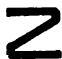
\includegraphics[keepaspectratio]{images/part002_1e1abfe7.jpg}}

A 是 Noether 环这一假设不能从陈述中略去（习题 2）。

定义 2. 设 A 是环。若 A-代数 R（未必交换）的每个元素都在 A 上是整的，则称 R 在 A 上是整的。若 R 是有限生成 A-模，则称 R 在 A 上是有限的。

由命题 1，每个有限 A-代数都是整的；若 R 是交换的且是有限 A-代数，则 R 显然是有限生成 A-代数；反之不真。

例（4）若 M 是有限生成 A-模，则 M 的自同态代数 \(\operatorname{End}_{\mathbf{A}}(\mathbf{M})\) 由 \((\mathrm{E}_{\mathrm{III}})\) 在 A 上是整的；特别地，对每个整数 n，矩阵代数 \(\mathbf{M}_{n}(\mathbf{A}) = \operatorname{End}_{\mathbf{A}}(\mathbf{A}^{n})\) 在 A 上是整的（甚至是有限的）。

命题 2. 设 A、A' 是两个环，R 是 A-代数，R' 是 A'-代数（未必交换），\(f\colon\mathbf{A}\to\mathbf{A}'\) 与 \(g\colon\mathbf{R}\to\mathbf{R}'\) 是两个环同态，使得图表

\pandocbounded{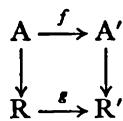
\includegraphics[keepaspectratio]{images/part002_4af46373.jpg}}

交换。若元素 \(x \in R\) 在 A 上是整的，则 \(g(x)\) 在 \(A'\) 上是整的。若 \(x^{n} + a_{1}x^{n-1} + \cdots + a_{n} = 0\) ，其中 \(a_{i} \in A\) （ \(1 \leqslant i \leqslant n\) ），我们推出

\[
(g (x)) ^ {n} + f \left(a _ {1}\right) (g (x)) ^ {n - 1} + \dots + f \left(a _ {n}\right) = 0.
\]

推论 1. 设 A 是环，B 是（交换）A-代数，C 是（未必交换）B-代数。那么在 A 上为整的每个元素 \(x \in \mathbf{C}\) 在 B 上也是整的。

推论 2. 设 K 是域，L 是 K 的扩域，x、\(x'\) 是 L 的两个在 K 上共轭的元素（《代数》，第 V 章，§ 6，第 2 节）。若 A 是 K 的子环且 x 在 A 上是整的，则 \(x'\) 也在 A 上是整的。

存在一个 K-同构 \(f\) ，它把 \(\mathbf{K}(x)\) 映到 \(\mathbf{K}(x')\) 上，使得 \(f(x) = x'\) ，且 \(\mathbf{A}\) 的元素在 \(f\) 下不变。

推论 3. 设 A 是环，B 是（交换）A-代数，C 是（未必交换）B-代数。若 C 在 A 上是整的，则 C 在 B 上是整的。

命题 3. 设 \((\mathbf{R}_i)_{1\leqslant i\leqslant n}\) 是（未必交换）的

A-代数的有限族，设 \(\mathbf{R} = \prod_{i=1}^{n} \mathbf{R}_i\) 是它们的乘积。要使元素 \(x = (x_i)_{1 \leq i \leq n}\) （\(\mathbf{R}\) 的）在 \(\mathbf{A}\) 上是整的，必须且只需每个 \(x_i\) 都在 \(\mathbf{A}\) 上是整的。要使 \(\mathbf{R}\) 在 \(\mathbf{A}\) 上是整的，必须且只需每个 \(\mathbf{R}_i\) 都在 \(\mathbf{A}\) 上是整的。

显然只需证明第一个断言。条件必要由命题 2 得出。反之，若每个 \(x_{i}\) 都在 \(A\) 上是整的，则子代数 \(A[x_{i}]\) （\(R_{i}\) 的）是有限生成 \(A\) -模，因而 R 的子代数 \(\prod_{i=1}^{n} \mathrm{A}[x_i]\) 也是；由于 \(\mathrm{A}[x]\) 含于这个子代数，由命题 1，\(x\) 在 A 上是整的。

命题 4. 设 A 是环，R 是 A-代数（未必交换），\((x_{i})_{1\leq i\leq n}\) 是 R 的两两可交换元素的有限族。若对所有 \(i, x_{i}\) 都在 \(A[x_{1},\cdots,x_{i-1}]\) 上是整的（特别地，若所有 \(x_{i}\) 都在 A 上是整的），则 R 的子代数 \(A[x_{1},\ldots,x_{n}]\) 是有限生成 A-模。

我们对 \(n\) 作归纳论证，命题就是 \((\mathbf{E}_{\mathrm{II}})\) （当 \(n = 1\) 时）。归纳假设蕴涵 \(B = A[x_{1}, \cdots, x_{n-1}]\) 是有限生成 A-模；由于 \(x_{n}\) 在 B 上是整的，\(B[x_{n}] = A[x_{1}, \cdots, x_{n}]\) 是有限生成 B-模，从而也是有限生成 A-模（《代数》，第 II 章，§ 1，第 13 节，命题 25）。

推论 1. 设 A 是环，R 是（交换）A-代数。R 中在 A 上为整的元素组成的集是 R 的一个子代数。

事实上，若 x, y 是 R 的两个在 A 上为整的元素，则由命题 4，A{[}x, y{]} 是有限生成 A-模；由于它含 \(x + y\) 与 xy，推论由命题 1 得出。

\pandocbounded{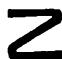
\includegraphics[keepaspectratio]{images/part002_90735efb.jpg}}

在非交换代数中，两个 A 上整元素的和与积未必在 A 上是整的（习题 4）。

推论 2. 设 A 是环，R 是 A-代数（未必交换），E 是 R 中两两可交换且在 A 上为整的元素组成的集。则 R 的由 E 生成的子 A-代数 B 在 A 上是整的。

B 的每个元素都属于 B 的一个由 E 的有限子集生成的子 A-代数。

注（3）由命题 4 推出，每个在 A 上为整的交换 A-代数都是 A 上有限子代数的一个右有向族的并。

命题 5. 设 A 是环，A' 与 R 是两个（交换）A-代数。若 R 在 A 上是整的，则 \(R \otimes_{A} A'\) 在 A' 上是整的。

考虑任一元素 \(x' = \sum_{i=1}^{n} x_i \otimes a_i'\) （\(\mathbf{R} \otimes_{\mathbf{A}} \mathbf{A}'\) 的），其中 \(x_i\) 属于 \(\mathbf{R}\) ，\(a_i'\) 属于 \(\mathbf{A}'\) ；由于 \(x_i \otimes a_i' = (x_i \otimes 1)a_i'\) 且诸 \(x_i \otimes 1\) 在 \(\mathbf{A}'\) 上是整的（命题 2），\(x\) 亦然。

推论. 设 R 是环，A、B、C 是 R 的子环，使得 \(A \subset B\) 。若 B 在 A 上是整的，则 C{[}B{]} 在 C{[}A{]} 上是整的。

\(B \otimes_{A} C[A]\) 由命题 5 在 \(C[A]\) 上是整的，因而典范像 \(C[B]\) （\(B \otimes_{A} C[A]\) 在 \(R\) 中的，R 视为 A-代数）由命题 2 也是。

命题 6. 设 A 是环，B 是（交换）A-代数，C 是（未必交换）B-代数。若 B 在 A 上是整的且 C 在 B 上是整的，则 C 在 A 上是整的。

只需验证每个 \(x \in C\) 在 A 上是整的。由假设存在一个系数在 B 中且以 x 为根的首一多项式 \(X^{n} + b_{1}X^{n-1} + \cdots + b_{n}\) ；于是 x 在 \(B' = A[b_{1}, \ldots, b_{n}]\) 上是整的，从而 \(B'[x]\) 是有限生成 \(B'\) -模。但由于 B 在 A 上是整的，\(B'\) 是有限生成 A-模（命题 4）；我们断定 \(\mathbf{B}'[x]\) 也是有限生成 A-模（《代数》，第 II 章，§1，第 13 节，命题 25），因而 \(x\) 在 \(\mathbf{A}\) 上是整的。

推论. 设 A 是环，R、R' 是两个在 A 上为整的（交换）A-代数。则 \(R \otimes_{A} R'\) 在 A 上是整的。

\(R \otimes_{A} R'\) 在 \(R'\) 上是整的（命题 5），因而结论由命题 6 得出。

\subsection{环的整闭包. 整闭整环}

定义 3. 设 A 是环，R 是（交换）A-代数。由 R 中在 A 上为整的元素组成的 R 的子 A-代数 A'（第 1 节，命题 4 的推论 1）称为 A 在 R 中的整闭包。若 A' 等于 A 在 R 中的典范像，则称 A 在 R 中是整闭的。

\textbf{注}\par

\begin{enumerate}
\def\labelenumi{(\arabic{enumi})}
\item
  若 \(h: \mathbf{A} \to \mathbf{R}\) 是定义 \(\mathbf{R}\) 上 A-代数结构的环同态，则 \(\mathbf{A}\) 在 \(\mathbf{R}\) 中的整闭包也是 \(h(\mathbf{A})\) 在 \(\mathbf{R}\) 中的整闭包。另一方面，若 \(\mathbf{R}'\) 是 \(\mathbf{R}\) 的子代数，则 \(\mathbf{A}\) 在 \(\mathbf{R}'\) 中的整闭包是 \(\mathbf{A}' \cap \mathbf{R}'\) 。
\item
  若 A 是域，则 A 在 R 中的整闭包 \(A'\) 由 R 中在 A 上为代数的元素组成（第 1 节，例 1）；把域扩张所用的术语（《代数》，第 V 章，§3，第 3 节）加以推广，\(A'\) 这时也称为域 A 在代数 R 中的代数闭包，且若 \(A' = A\) ，称 A 在 R 中是代数闭的。
\end{enumerate}

定义 4. 若 A 是整环，则 A 在其分式域中的整闭包称为 A 的整闭包。若整环等于它的整闭包，则称它是整闭的。

\pandocbounded{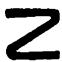
\includegraphics[keepaspectratio]{images/part002_6bc214f1.jpg}}

注意，整闭的整环未必在包含它的任何环中都是闭的，正如一个非代数闭的域这一例子所示。

命题 7. 设 A 是环，R 是 A-代数。A 在 R 中的整闭包 A' 是 R 中整闭的子环。

A' 在 R 中的整闭包由第 1 节命题 6 在 A 上是整的；因此它等于 A'。

推论. 整环 A 的整闭包是整闭的整环。

设 K 是 A 的分式域，B 是 A 的整闭包。显然

K 是 B 的分式域，只需把命题 7 应用于 R = K。

命题 8. 设 R 是环，\((\mathbf{B}_{\lambda})_{\lambda \in \mathbf{L}}\) 是 R 的子环族，且对每个 \(\lambda \in L\) ，设 \(A_{\lambda}\) 是 \(B_{\lambda}\) 的子环。若每个 \(A_{\lambda}\) 在 \(B_{\lambda}\) 中是整闭的，则 \(A = \bigcap_{\lambda \in L} A_{\lambda}\) 在 \(B = \bigcap_{\lambda \in L} B_{\lambda}\) 中是整闭的。

这由定义 3 及第 1 节命题 2 的推论 1 立即得出。

推论. 整环 A 的整闭子整环的非空族的每个交都是整闭的整环。

只需应用命题 8，取 R 与诸 \(B_{\lambda}\) 等于 A 的分式域 K，并注意 K 的在 K 中整闭的子环更是整闭的整环，因为其分式域含于 K。

命题 9. 设 A 是环，\((\mathbf{R}_i)_{1 \leqslant i \leqslant n}\) 是 A-代数的有限族，\(\mathbf{A}_i'\) 是 A 在 \(\mathbf{R}_i\) 中的整闭包（ \(1 \leqslant i \leqslant n\) ）。则 A 在 \(\mathbf{R} = \prod_{i=1}^{n} \mathbf{R}_i\) 中的整闭包等于 \(\prod_{i=1}^{n} \mathbf{A}_i'\) 。

这是第 1 节命题 3 的直接推论。

推论 1. 设 A 是既约 Noether 环，\(\mathfrak{p}_i\) （ \(1 \leqslant i \leqslant n\) ）是它的互异极小素理想，\(\mathbf{K}_i\) 是整环 \(\mathbf{A} / \mathfrak{p}_i\) 的分式域（典范同构于局部环 \(\mathbf{A}_{\mathfrak{p}_i}\) （第 IV 章，§2，第 5 节，命题 10）），\(\mathbf{A}_i'\) 是 A 在 \(\mathbf{K}_i\) 中的整闭包（ \(1 \leqslant i \leqslant n\) ）。则 A 的全分式环 B 到 \(\prod_{i=1}^{n} \mathbf{K}_i\) （出处同上）上的典范同构把 A 在 B 中的整闭包映到积环 \(\prod_{i=1}^{n} \mathbf{A}_i'\) 上。

推论 2. 要使既约 Noether 环在其分式环中是整闭的，必须且只需它是整闭（Noether）整环的直合成。

\subsection{整闭整环的例子}

命题 10. 每个主理想整环都是整闭的。\par

设 A 是主理想整环，K 是它的分式域，x 是 K 的元素。存在 A 的两个互素元素 a, b 使得 \(x = ab^{-1}\) （《代数》，第 VII 章，§1，第 2 节，命题 1 及第 VI 章，§1，第 11 节，命题 9 (DIV)）。若 x 在 A 上是整的，则它是一个多项式的根

\(X^{n} + c_{1}X^{n-1} + \cdots + c_{n}\) （A{[}X{]} 中的）。于是 \(a^{n} = b(-c_{1}a^{n-1} - \cdots - c_{n}b^{n-1})\) ，这证明 \(b\) 整除 \(a^{n}\) 。由于 \(a\) 与 \(b\) 互素，这蕴涵 \(b\) 在 A 中可逆（《代数》，第 VI 章，§ 1，第 12 节，命题 11 的推论 1 (DIV)）；从而 \(x \in A\) 。

引理 2. 设 R 是环，P 是 R{[}X{]} 中的首一多项式。存在一个含 R 的环 R'，使得在多项式环 R'{[}X{]} 中多项式 P 是次数为 1 的首一多项式的乘积。

我们对 \(n\) （\(\mathbf{P}\) 的次数）作归纳，引理对 \(n = 0\) 与 \(n = 1\) 是显然的。于是设 \(n > 1\) 。设 \(\mathfrak{a}\) 是 \(\mathbb{R}[\mathbf{X}]\) 中由 \(\mathbf{P}\) 生成的理想，设 \(f\) 是 \(\mathbb{R}[\mathbf{X}]\) 到 \(\mathbf{B} = \mathbb{R}[\mathbf{X}] / \mathfrak{a}\) 上的典范同态。由于 \(\mathbf{P}\) 是首一的，对每个多项式 \(\mathbf{Q} \in \mathbb{R}[\mathbf{X}]\) ，\(\deg(\mathrm{PQ}) = \deg(\mathrm{P}) + \deg(\mathrm{Q})\) ，由此 \(\mathfrak{a} \cap \mathbb{R} = 0\) ；\(f\) 在 \(\mathbb{R}\) 上的限制因而是单射。把 \(\mathbb{R}\) 与子环 \(f(\mathbb{R})\) （\(\mathbb{B}\) 的）借助 \(f\) 等同起来，并写 \(b = f(\mathbf{X})\) ，我们看到 \(b\) 是 \(\mathbf{P}\) 在 \(\mathbb{B}\) 中的根，这里 \(\mathbf{P}\) 视为 \(\mathbb{B}[\mathbf{X}]\) 中的多项式。于是存在首一多项式 \(\mathbf{Q}\) （在 \(\mathbb{B}[\mathbf{X}]\) 中，次数为 \(n - 1\)）使得 \(\mathrm{P}(\mathbf{X}) = (\mathbf{X} - b)\mathrm{Q}(\mathbf{X})\) （《代数》，第 IV 章，§ 1，第 4 节，命题 5）。由归纳假设，存在环 \(\mathbb{R}' \supseteq \mathbb{B}\) 使得在 \(\mathbb{R}'[\mathbf{X}]\) 中多项式 \(\mathbf{Q}\) 是次数为 1 的首一多项式的乘积；显然在 \(\mathbb{R}'[\mathbf{X}]\) 中 \(\mathbf{P}\) 这时是次数为 1 的首一多项式的乘积。

命题 11. 设 A 是环，R 是 A-代数，P 与 Q 是 R{[}X{]} 中的首一多项式。若 PQ 的系数都在 A 上是整的，则 P 与 Q 的系数都在 A 上是整的。

两次应用引理 2，我们看出存在一个环 \(\mathbf{R}'\) （含 \(\mathbf{R}\)）以及元素族 \((a_i)_{1 \leqslant i \leqslant m}, (b_j)_{1 \leqslant j \leqslant n}\) （\(\mathbf{R}'\) 的），使得在 \(\mathbf{R}'[\mathbf{X}]\) 中 \(\mathrm{P}(\mathbf{X}) = \prod_{i=1}^{m} (\mathbf{X} - a_i)\) ，\(\mathbf{Q}(\mathbf{X}) = \prod_{j=1}^{n} (\mathbf{X} - b_j)\) ；\(\mathbf{PQ}\) 的系数属于整闭包 \(\mathbf{A}'\) （\(\mathbf{A}\) 在 \(\mathbf{R}'\) 中的），因而（第 2 节，命题 7）元素 \(a_i\) （ \(1 \leqslant i \leqslant m\) ）与 \(b_j\) （ \(1 \leqslant j \leqslant n\) ）属于 \(\mathbf{A}'\) 。由此得出 \(\mathbf{P}\) 与 \(\mathbf{Q}\) 的系数在 \(\mathbf{A}\) 上是整的（第 1 节，命题 4 的推论 1）。

设 A 是整环，K 是它的分式域，\(K'\) 是 K-代数（未必交换）。给定一个在 K 上为代数的元素 \(x \in K'\) ，多项式 \(P \in K[X]\) （满足 \(P(x) = 0\) 者）组成一个理想 \(a \neq 0\) （\(K[X]\) 的） ，它必然是主理想（《代数》，第 IV 章，§1，第 5 节，命题 7）。存在唯一的首一多项式生成 a；把《代数》第 V 章，§3，第 1 节，定义 3 中引入的术语加以推广，这个首一多项式将称为 x 在 K 上的极小多项式。

推论. 设 A 是整环，K 是它的分式域，x 是 K-代数 \(K'\) （未必交换）的元素。若 x 在 A 上是整的，则 x 在 K 上的极小多项式 P 的系数在 A 上是整的（从而若 A 是整闭的，它们属于 A）。

由假设（第 1 节，定理 1）存在一个首一多项式 \(Q \in A[X]\) 使得 \(Q(x) = 0\) 。由于 P 在 K{[}X{]} 中整除 Q，由命题 11，P 的系数在 A 上是整的。

设 A 是环，R 是（交换）A-代数；定义 R 上 A-代数结构的同态 \(\phi: A \rightarrow R\) 可以唯一地扩张为 A 与 R 上的多项式环的同态 \(A[X] \rightarrow R[X]\) ，它保持 X 不变，从而 \(R[X]\) 具有一个典范的 A{[}X{]}-代数结构。

命题 12. 设 A 是环，R 是 A-代数，P 是 \(R[X_{1},\ldots,X_{n}]\) 中的多项式。要使 P 在 \(A[X_{1},\ldots,X_{n}]\) 上是整的，必须且只需 P 的系数在 A 上是整的。

把 \(R[X_{1},\ldots,X_{n}]\) 中的多项式视为关于 \(X_{n}\) 的多项式（系数在 \(R[X_{1},\ldots,X_{n-1}]\) 中），我们立即看出可化归为对 n=1 证明本命题。设 P 是 \(R[X]\) 中的多项式；由第 1 节命题 5 立即得出，若 P 的系数属于 A 在 R 中的整闭包 B，则属于 \(B[X]=B\otimes_{A}A[X]\) 的元素 P 在 A{[}X{]} 上是整的。反之，设 P 在 A{[}X{]} 上是整的，并设

\[
\mathrm{Q} (\mathrm{Y}) = \mathrm{Y} ^ {m} + \mathrm{F} _ {1} \mathrm{Y} ^ {m - 1} + \dots + \mathrm{F} _ {m}
\]

是系数为 \(F_{i} \in A[X]\) 且以 P 为根的首一多项式。设 r 是一个严格大于多项式 P 与 \(F_{i}\) （ \(1 \leqslant i \leqslant m\) ）的所有次数的整数，我们写

\[
\mathrm{P} _ {1} (\mathrm{X}) = \mathrm{P} (\mathrm{X}) - \mathrm{X} ^ {r}.
\]

于是 \(\mathbf{P}_1\) 是多项式

\[
\mathrm{Q} _ {1} (\mathrm{Y}) = \mathrm{Q} (\mathrm{Y} + \mathrm{X} ^ {r}) = \mathrm{Y} ^ {m} + \mathrm{G} _ {1} \mathrm{Y} ^ {m - 1} + \dots + \mathrm{G} _ {m}
\]

系数在 A{[}X{]} 中；因此我们可以写

\[
- \mathrm{P} _ {1} (\mathrm{P} _ {1} ^ {m - 1} + \mathrm{G} _ {1} \mathrm{P} _ {1} ^ {m - 2} + \dots + \mathrm{G} _ {m - 1}) = \mathrm{G} _ {m}.\tag{1}
\]

现在 \(r\) 的选取蕴涵 \(-\mathbf{P}_1\) 是 \(\mathbb{R}[\mathbf{X}]\) 中的首一多项式，\(\mathbf{G}_m(\mathbf{X}) = \mathbf{Q}(\mathbf{X}^r)\) 亦然，因为多项式 \(\mathrm{F}_k(\mathbf{X})\mathbf{X}^{r(m - k)}\) 的次数都 \(< rm\) （对 \(k \geqslant 1\) ）。我们首先断定多项式

\[
\mathrm{P} _ {1} ^ {m - 1} + \mathrm{G} _ {1} \mathrm{P} _ {1} ^ {m - 2} + \dots + \mathrm{G} _ {m - 1}
\]

（R{[}X{]} 中的）也是首一的；此外，由于 \(G_{m}\) 的系数属于 A，命题 11 表明 \(P_{1}\) 的系数在 A 上是整的，因而 P 的系数当然在 A 上是整的。

命题 13. 设 A 是环，R 是 A-代数，A' 是 A 在 R 中的整闭包。则 A{[}X₁, \ldots, Xₙ{]} 在 R{[}X₁, \ldots, Xₙ{]} 中的整闭包等于 A'{[}X₁, \ldots, Xₙ{]}。

这由命题 12 及第 2 节的定义 3 得出。

推论 1. 设 A 是整环，A' 是它的整闭包。则多项式环 A{[}X₁, \ldots, Xₙ{]} 的整闭包是 A'{[}X₁, \ldots, Xₙ{]}。

对 n 作归纳论证，问题立即化归为 n = 1 的情形。设 K 是 A 的分式域，它也是 A' 的分式域；若 A{[}X{]} 的分式域 K(X) 的元素 P 在 A{[}X{]} 上是整的，则它属于多项式环 K{[}X{]} ，因为后者是主理想整环（《代数》，第 IV 章，§ 1，第 5 节，命题 7）从而是整闭的（命题 10）；于是推论由应用于 R = K 的命题 13 得出。

推论 2. 设 A 是整环。要使多项式环 A{[}X \(_{1}\) , \ldots, X \(_{n}\) {]} 是整闭的，必须且只需 A 是整闭的。

推论 3. 若 K 是域，则每个多项式代数 \(\mathbf{K}[\mathbf{X}_1,\ldots ,\mathbf{X}_n]\) 都是整闭的整环。

\subsection{完全整闭整环}

定义 5. 若整环 A 满足下列条件，则称它是完全整闭的：A 的分式域 K 中每个使得所有幂 \(x^{n}\) （ \(n \geqslant 0\) ）都含于 K 的一个有限生成子 A-模的元素 x 属于 A。

注意，诸 \(x^n\) 含于 K 的一个有限生成子 A-模这一假设也可以表述为：存在非零元素 \(d \in \mathbf{A}\) 使得 \(dx^n \in \mathbf{A}\) 对所有 \(n \geqslant 0\) 成立；因为后一条件意味着 \(x^n \in \mathrm{Ad}^{-1}\) ；反之，若 \((b_i)_{1 \leqslant i \leqslant m}\) 是 K 的元素的有限序列，则存在 \(d \in \mathbf{A}\) 使得 \(db_i \in \mathbf{A}\) 对 \(1 \leqslant i \leqslant m\) 成立，从而 \(d\mathbf{M} \subset \mathbf{A}\) 对由诸 \(b_i\) 生成的 K 的子 A-模 M 成立。

显然完全整闭的整环是整闭的；反之，第 1 节命题 1 的推论表明整闭的 Noether 整环是完全整闭的。* 另一方面，高 ≥ 2 的赋值的环（第 VI 章，§ 4，第 4 节）是整闭的但不是完全整闭的。* 若 (A\_t) 是有相同分式域 K 的完全整闭整环的族，则 A = ∩\_t A\_t 是完全整闭的。因为若 x ∈ K 使得对 A 中某个非零 d，\(dx^n\) 对所有 n \textgreater{} 0 属于 A，则假设蕴涵 x ∈ A\_t 对所有 t 成立，从而 x ∈ A。

命题 14. 设 A 是完全整闭的整环。则每个多项式环 \(\mathbf{A}[\mathbf{X}_1,\ldots ,\mathbf{X}_n]\) （相应地，每个形式幂级数环 \(\mathbf{A}[[\mathbf{X}_1,\dots ,\mathbf{X}_n]]\) ）是完全整闭的。

对 \(n\) 作归纳，只需证明 A{[}X{]} （相应地 A{[}{[}X{]}{]}）是完全整闭的。设 P 是 A{[}X{]} （相应地 A{[}{[}X{]}{]}）的分式域的元素，并设存在非零元素 Q ∈ A{[}X{]} （相应地 Q ∈ A{[}{[}X{]}{]}）使得 QP \(^{m}\) ∈ A{[}X{]} （相应地 QP \(^{m}\) ∈ A{[}{[}X{]}{]}）对每个整数 m ≥ 0 成立。若 K 是 A 的分式域，则 A{[}X{]} （相应地 A{[}{[}X{]}{]}）是 K{[}X{]} （相应地 K{[}{[}X{]}{]}）的子环，而 K{[}X{]} （相应地 K{[}{[}X{]}{]}）是主理想整环（《代数》，第 VII 章，§ 1，第 1 节）从而是整闭的（第 4 节，命题 10）且是 Noether 的（《代数》，第 VIII 章，§ 2，第 3 节），因此是完全整闭的；于是我们已经看到 \(\mathbf{P} \in \mathbf{K}[\mathbf{X}]\) （相应地 \(\mathbf{P} \in \mathbf{K}[[\mathbf{X}]]\) ）。设 \(\mathbf{P} = \sum_{k=0}^{\infty} a_k \mathbf{X}^k\) （ \(a_k \in \mathbf{K}\) ）与 \(\mathbf{Q} = \sum_{k=0}^{\infty} b_k \mathbf{X}^k\) （ \(b_k \in \mathbf{A}\) ），我们用反证法论证，设诸 \(a_k\) 并非都属于 \(\mathbf{A}\) ；于是有一个最小的指标 \(i\) 使 \(a_i \notin \mathbf{A}\) ；若我们写

\(P_{1}=\sum_{k=0}a_{k}X^{k}\in A[X]\) ，则由假设立即得出 \(Q(P-P_{1})^{m}\in A[X]\) （相应地 \(Q(P-P_{1})^{m}\in A[[X]]\) ）对所有 \(m\geqslant0\) 也成立。设 j 是使 \(b_{j}\neq0\) 的最小整数；显然在 \(Q(P-P_{1})^{m}\) 中系数 \(\neq0\) 的最低次项是 \(b_{j}a_{i}^{m}X^{j+m^{i}}\) ，因而 \(b_{j}a_{i}^{m}\in A\) 对所有 \(m\geqslant0\) 成立；但由于 A 是完全整闭的，这蕴涵 \(a_{i}\in A\) ，与假设相反。

命题 15. 设 A 是一个带滤链的环，其滤链是穷竭的，且 A 的每个主理想对于由该滤链定义的拓扑是闭的。若相伴分次环 gr(A)（第 III 章，§2，第 3 节）是完全整闭的整环，则 A 是完全整闭的整环。

设 \((\mathbf{A}_n)_{n\in \mathbf{Z}}\) 是 \(\mathbf{A}\) 上定义的滤链；由于 \(\bigcap_{n\in \mathbf{Z}}\mathbf{A}_n\) 是理想 (0) 的闭包（第 III 章，§ 2，第 5 节），假设首先蕴涵滤链 \((\mathbf{A}_n)\) 是分离的，且由于 \(\operatorname{gr}(\mathbf{A})\) 是整环，\(\mathbf{A}\) 也是整环（第 III 章，§ 2，第 3 节，命题 1 的推论）。设 \(x = b / a\) 是分式域 \(\mathbf{K}\) （\(\mathbf{A}\) 的）的元素（ \(a\in \mathbf{A}, b\in \mathbf{A}\) ），对它存在元素 \(d\neq 0\) （\(\mathbf{A}\) 的），使得 \(dx^n\in \mathbf{A}\) 对所有 \(n\geqslant 0\) 成立。我们必须证明 \(b\in \mathbf{A}a\) ，且由假设理想 \(\mathbf{A}a\) 是闭的，只需证明对所有 \(n\in \mathbf{Z}, b\in \mathbf{A}a + \mathbf{A}_n\) 。由于 \(\mathbf{A}\) 的滤链是穷竭的，存在整数 \(q\in \mathbf{Z}\) 使得 \(b\in \mathbf{A}a + \mathbf{A}_q\) 。因此只需证明关系 \(b\in \mathbf{A}a + \mathbf{A}_m\) 蕴涵 \(b\in \mathbf{A}a + \mathbf{A}_{m + 1}\) 。

设 \(b = ay + z\) ，其中 \(y \in \mathbf{A}\) ，\(z \in \mathbf{A}_m\) 。则由假设 \(dx^n \in \mathbf{A}\) 对所有 \(n \geqslant 0\) 成立，由此立即得到 \(d(x - y)^n \in \mathbf{A}\) 对所有 \(n \geqslant 0\) 成立；换句话说，\(dz^n = a^n t_n\) ，其中 \(t_n \in \mathbf{A}\) 对所有 \(n \geqslant 0\) 成立。我们显然可只限于 \(z \neq 0\) 的情形。设 \(v\) 表示 \(\mathbf{A}\) 上的阶函数（第 III 章，§1，第 2 节），我们写 \(v(d) = n_1\) ，\(v(z) = n_2 \geqslant m\) ，\(v(a) = n_3\) ；设 \(d', z', a'\) 分别是 \(d, z, a\) 在 \(\mathbf{A}_{n_1}/\mathbf{A}_{n_1+1}\) 、\(\mathbf{A}_{n_2}/\mathbf{A}_{n_2+1}\) 、\(\mathbf{A}_{n_3}/\mathbf{A}_{n_3+1}\) 中的像。对所有 \(n \geqslant 0\) ，\(v(dz^n) = n_1 + nn_2\) （第 III 章，§2，第 3 节，命题 1），因而 \(\mathrm{gr}(\mathbf{A})\) 中 \(dz^n\) 的典范像是 \(d'z'^n\) ；同样可看出 \(\mathrm{gr}(\mathbf{A})\) 中 \(a^n t_n\) 的典范像形如 \(a'^n t_n'\) ，其中 \(t_n' \in \mathrm{gr}(\mathbf{A})\) ，且由于 \(a' \neq 0\) ，我们推出对所有 \(n \geqslant 0\) ，\(d'(z'/a')^n \in \mathrm{gr}(\mathbf{A})\) 。\(\mathrm{gr}(\mathbf{A})\) 完全整闭这一假设因此蕴涵存在 \(s' \in \mathrm{gr}(\mathbf{A})\) 使得 \(z' = a's'\) ；把 \(s'\) 分解为齐次元素之和，进一步可看出（由于 \(z'\) 与 \(a'\) 是齐次的）\(s'\) 可假设是齐次的，即某个 \(s \in \mathbf{A}\) 的像；于是 \(v(as) = v(z) = n_2\) 且 \(z \equiv as (\mathrm{mod. A_{n_2+1}})\) ；由于 \(n_2 \geqslant m\) ，更有 \(z \equiv as (\mathrm{mod. A_{m+1}})\) ，从而 \(b \equiv a(y + s) (\mathrm{mod. A_{m+1}})\) 。
